\documentclass[12pt]{article}

\usepackage[a4paper,margin=1in]{geometry}
\usepackage[T1]{fontenc}
\usepackage[utf8]{inputenc}
\usepackage{lmodern}
\usepackage{microtype}
\usepackage{graphicx}
\usepackage{booktabs}
\usepackage{longtable}
\usepackage{array}
\usepackage{calc}
\usepackage{algorithm}
\usepackage{algpseudocode}
\usepackage{hyperref}

\providecommand{\tightlist}{%
  \setlength{\itemsep}{0pt}\setlength{\parskip}{0pt}}

\title{CellSAM Adaptation for hiPSC-CM Instance Segmentation}
\author{Author Name}
\date{\today}

\begin{document}

\maketitle
\begin{abstract}
This thesis studies whole-cell instance segmentation of human hiPSC-derived cardiomyocytes in dense microscopy images with weak boundaries and strong cell-cell adhesion. We start from the released CellSAM checkpoint and perform an implementation-level audit to establish a reproducible segmentation branch and a unified final inference protocol. On top of this audited basis, we build a cardiomyocyte-specific adaptation framework with decoder-focused fine-tuning, biology-prior-aware channel handling, and explicit separation between Oracle and end-to-end evaluation. The sealed segmentation mainline is T28, reported by dual-seed mean on val71 (PQ@0.5 = 0.6837, BM-Dice = 0.8166), while locked test73 baselines are retained as a split-aware reference tier. For deployment, the selected detector-segmentation route is T33g(dapi\_cm, candidate-aligned, q35) + T28, framed as a biology-prior line rather than a detector-metric-optimal claim. The analysis indicates that the current deployment bottleneck is prompt quality rather than mask-decoder capacity. Overall, this work provides a domain-audited and prompt-aware adaptation framework for foundation segmentation in challenging cardiomyocyte imaging.

\end{abstract}
\clearpage
\tableofcontents

% !TEX root = ../main.tex
\section{Introduction}\label{introduction}

\subsection{Problem Background}\label{problem-background}

Instance segmentation of cardiomyocytes is a prerequisite for many downstream analyses in stem-cell-based cardiac research, including morphology profiling, maturation assessment, drug response analysis, and phenotypic screening. In this thesis, the target domain is specifically the Allen Institute dataset of \textbf{human hiPSC-derived cardiomyocytes} \cite{rafelski2024allen}. This scope matters. The thesis does not study generic cell segmentation, and it does not currently claim transfer to mouse cardiomyocytes or to other cardiac imaging settings.

From a modeling perspective, this is a difficult segmentation problem. Cardiomyocytes are highly variable in size, elongated rather than round, densely packed, and often exhibit weak or ambiguous boundaries in brightfield imaging. These properties make whole-cell instance segmentation harder than standard nucleus segmentation and less compatible with methods that assume compact, convex, or well-separated object shapes.

Recent foundation models have changed the landscape of image segmentation. Segment Anything Model (SAM) demonstrated that large-scale pretraining can produce highly transferable segmentation representations \cite{kirillov2023sam}, and CellSAM extended this idea to the cell-imaging domain \cite{israel2024cellsam}. Nevertheless, transfer across biological imaging tasks is still not automatic. The released CellSAM checkpoint was not trained specifically for hiPSC-derived cardiomyocytes, and cardiomyocyte morphology differs substantially from the cell types that dominate most public microscopy benchmarks. As a result, the central question of this thesis is not whether CellSAM is useful in general, but whether a released cell foundation model can be adapted into a domain-audited, prompt-aware, cardiomyocyte-specific segmentation system that remains scientifically traceable.

\subsection{Challenges}\label{challenges}

The project faces three coupled challenges.

First, the task itself is structurally difficult. Whole-cell boundaries are weak, neighboring cells may touch or overlap, and nucleus-centered cues do not fully define cell extent. A model can therefore appear reasonable at semantic foreground level while still failing at instance separation.

Second, the released CellSAM artifact is not a trivial baseline. It contains multiple internal branches, and the practical meaning of released-checkpoint segmentation inference cannot be taken directly from the paper wording alone. Before fair comparison or fine-tuning, the released checkpoint has to be audited as a software artifact.

Third, the deployment setting is prompt-limited. Under Oracle prompts, the current segmentation branch is already strong. Under automatically generated prompts, performance drops substantially. This means the main open problem is no longer only how to optimize mask quality under perfect boxes, but how to handle prompt-quality mismatch between training and deployment.

\subsection{Research Questions and Contributions}\label{research-questions-and-contributions}

This thesis is organized around three research questions.

\begin{enumerate}
\def\labelenumi{\arabic{enumi}.}
\tightlist
\item
  Can a released cell-domain foundation model be adapted into a strong human hiPSC-cardiomyocyte segmentation system?
\item
  How much do implementation-path choice and evidence-tier discipline affect the interpretation of CellSAM-based results?
\item
  Is the current performance bottleneck mainly the segmentation branch itself, or the quality of prompts supplied to it?
\end{enumerate}

The current evidence already supports a clear high-level answer, but only under split-aware reporting. The sealed segmentation mainline is T28 with dual-seed mean on \texttt{val71} (\texttt{PQ\ =\ 0.6837}, \texttt{BM-Dice\ =\ 0.8166}). As a locked reference tier, the historical single-checkpoint \texttt{test73} T27a result (\texttt{PQ\ =\ 0.659}, \texttt{BM-Dice\ =\ 0.800}, \texttt{AJI\ =\ 0.669}) remains useful for cross-baseline context. The Oracle-to-end-to-end gap further shows that the current project should be framed as \textbf{Oracle-strong but prompt-limited}.

This claim is strengthened by the fact that the baseline family is not weakly chosen. The comparison set includes a strong generalist cell segmenter (Cellpose \cite{stringer2021cellpose}), generic promptable segmentation (SAM ViT-B \cite{kirillov2023sam}), released cell-domain zero-shot transfer (CellSAM pretrained \cite{israel2024cellsam}), and a strong external medical foundation baseline (MedSAM \cite{ma2024medsam}). Therefore, the thesis is not arguing only that one tuned model beats an easy comparator. It argues that a carefully adapted cardiomyocyte pipeline can outperform four distinct and methodologically meaningful comparison axes.

Within that framing, the value of the work is stronger than a simple ``higher PQ'' statement. The thesis makes three main methodological contributions and one supporting reproducibility contribution.

\begin{enumerate}
\def\labelenumi{\arabic{enumi}.}
\tightlist
\item
  It develops \textbf{domain-aware input handling} for non-RGB cardiomyocyte microscopy, treating channel design as a biological and methodological problem rather than assuming natural-image RGB semantics.
\item
  It establishes \textbf{prompt-quality-aware fine-tuning} by separating Oracle GT-box conditions from detector-conditioned deployment, thereby identifying prompt mismatch rather than mask-decoder capacity as the main current bottleneck and motivating noisy-box adaptation as the correct next step.
\item
  It integrates \textbf{biology priors with foundation segmentation}, using DAPI for localization cues and Actn2 for cardiomyocyte structural identity instead of relying only on nuclei or generic off-the-shelf cell assumptions.
\item
  It contributes a code-level audit of the released CellSAM artifact together with a split-aware evidence hierarchy that separates locked \texttt{test73} results, \texttt{val71} supplementary analyses, and provisional single-seed observations.
\end{enumerate}

\subsection{Thesis Overview}\label{thesis-overview}

The remainder of the thesis is organized as follows. Section 2 reviews the biomedical and technical background of the task and summarizes the architecture principles of CellSAM, Cellpose, and MedSAM in this cardiomyocyte setting. Section 3 introduces the Allen hiPSC-cardiomyocyte dataset and formal metric definitions with split-aware reporting rules. Section 4 describes the final methodology, including preprocessing, detector-to-segmenter integration, postprocessing, and T28 training setup. Section 5 presents the main results, including the T28 mainline summary, split-aware reference comparisons, and detector-limited end-to-end analysis. Section 6 discusses methodological limits, evidence boundaries, and follow-up directions. The appendices provide parameter-level checkpoint-audit details and supplementary exploratory evidence.

\section{Background and Related Work}\label{background-and-related-work}

\subsection{Biomedical Background of the Task}\label{biomedical-background-of-the-task}

Human induced pluripotent stem cell-derived cardiomyocytes (hiPSC-CMs) are widely used as an in vitro model for cardiac biology, disease modeling, and phenotypic screening \cite{ahmed2020hipscm_maturation}. In these applications, the morphology of individual cells is not a cosmetic detail: it is closely tied to questions about maturation state, structural organization, drug response, and culture quality. This is one of the reasons why a cell-level segmentation task is meaningful in the first place. The goal is not merely to detect whether cardiomyocytes are present, but to recover individual cell extents in a way that supports downstream quantitative analysis.

Compared with many standard microscopy benchmarks, cardiomyocytes are structurally awkward segmentation targets. They are often elongated, anisotropic, irregular in width, and densely packed. Neighboring cells can touch or partially overlap in projection, while local boundaries may be weak in brightfield imaging. As a result, the object of interest is visually more complex than round or nucleus-like cells, and the mismatch between ``where a cell is'' and ``what its full outline should be'' is larger than in many easier segmentation settings.

This scope also sets an important boundary for the thesis. The current dataset and all locked results concern \textbf{human hiPSC-derived cardiomyocytes}. Therefore, the claims made in this thesis should be read as human hiPSC-CM claims. Possible transfer to mouse cardiomyocytes is scientifically interesting, but it remains a future adaptation question rather than a present conclusion of this work.

\subsection{Human--Mouse Transfer Boundary and Species-Specific Differences}\label{human-mouse-transfer-boundary-and-species-specific-differences}

The practical transfer question is not whether human-to-mouse adaptation is imaginable, but whether current human hiPSC-CM evidence can be extrapolated without species-aware adjustment. Existing evidence suggests this is unsafe: rodents and humans differ in electrophysiology and ion-channel dominance \cite{joukar2021rodent_human_ecg}, while hiPSC-CMs are typically immature relative to adult cardiomyocytes \cite{ahmed2020hipscm_maturation}. Cardiac single-cell and spatial-omics reviews further emphasize species-dependent cellular composition and cardiomyocyte state differences that affect interpretation across species \cite{palmer2024cardiac_omics}. A detailed species-gap summary is provided in Appendix~\ref{scope-and-transfer-notes}.

Therefore, the thesis treats mouse transfer as a future adaptation track rather than a supported claim of direct zero-shot reuse. Any credible transfer route should include at least: (i) mouse-domain zero-shot audit, (ii) detector-prior retuning, and (iii) mouse-specific decoder fine-tuning under the same split-aware evaluation protocol.

\subsection{Imaging Modalities and Structural Cues}\label{imaging-modalities-and-structural-cues}

The Allen hiPSC-CM dataset used in this thesis combines several channels with different biological meanings. Brightfield provides the main low-cost imaging modality and is central to the deployment-oriented question of this thesis, but it also gives the weakest boundary information. The alpha-Actinin2 channel highlights sarcomeric or cytoskeletal structure inside cardiomyocytes, which is highly informative for cell identity and internal organization but does not directly provide a clean whole-cell contour. The DAPI channel highlights nuclei and is therefore useful for localization, yet a nucleus is only a proxy for a whole cardiomyocyte and not its full spatial extent.

These channels are therefore complementary rather than interchangeable. Brightfield is attractive because it is broadly available and less burdensome than fluorescence-heavy acquisition. Actn2 provides rich structural information about cardiomyocyte organization. DAPI provides a strong positional prior for candidate cells. The central challenge is that none of these signals alone perfectly defines the whole-cell boundary, which is why both detection quality and segmentation quality must be considered jointly in this project.

From the perspective of method design, these channel semantics are not merely descriptive background. They define the biological priors that motivate the pipeline itself. DAPI provides a localization prior for candidate-cell prompting, while Actn2 provides a cardiomyocyte-specific structural prior that helps distinguish true cardiomyocyte extent from generic brightfield texture. This is why the thesis treats channel handling and prompt construction as part of the method rather than as minor preprocessing details.

\subsection{Why Whole-Cell Instance Segmentation Is Difficult in Cardiomyocytes}\label{why-whole-cell-instance-segmentation-is-difficult-in-cardiomyocytes}

The present thesis focuses on whole-cell instance segmentation rather than nucleus segmentation or semantic foreground extraction. This choice is important biologically and methodologically. A nucleus-level mask is insufficient for morphology analysis, and a semantic foreground mask can overestimate performance by merging adjacent cells into a single blob. For cardiomyocytes, this failure mode is particularly plausible because elongated neighboring cells can align, touch, or overlap in ways that make the global foreground look reasonable while the instance structure is wrong.

This difficulty also explains several design choices in the project. DAPI-based detection can provide candidate boxes, but nuclear localization does not resolve the full cell boundary. Structural channels such as Actn2 can provide clues about internal organization, but they do not automatically separate touching cells. Brightfield imaging is the most practical modality for future deployment, but its weak boundaries make direct whole-cell delineation difficult. The thesis therefore studies a prompt-based segmentation pipeline in which localization and per-cell mask prediction are treated as related but distinct problems.

\subsection{Foundation Models for Interactive Segmentation}\label{foundation-models-for-interactive-segmentation}

Segment Anything Model (SAM) established a new paradigm for promptable segmentation by combining a Vision Transformer image encoder, a prompt encoder, and a lightweight mask decoder \cite{kirillov2023sam}. Its main contribution was not a single-task architecture, but a reusable segmentation representation learned from large-scale pretraining. For biomedical imaging, this idea is attractive because annotation is expensive, morphology is diverse, and many applications require transferring a model across domains with limited labeled data.

However, direct transfer from natural-image pretraining to microscopy is not guaranteed to work well. Microscopy images differ in texture, intensity statistics, scale, and object structure. In particular, cardiomyocytes are long, anisotropic, and densely arranged, which violates many of the geometric assumptions that make generic segmentation models perform well on more regular biological objects. This motivates domain-specific adaptation rather than direct reuse of a released checkpoint.

\subsection{CellSAM and the Problem of Released-Checkpoint Semantics}\label{cellsam-and-the-problem-of-released-checkpoint-semantics}

CellSAM extends SAM to the cell segmentation domain by combining a detection branch and a segmentation branch \cite{israel2024cellsam}. Conceptually, its published methodology describes a two-stage pipeline: first learning cell detection, then adapting the segmentation branch. In practice, however, a released checkpoint is not only a scientific object but also a software object. The exact meaning of ``shared backbone'', ``stage 2 branch'', or released inference branch semantics must be verified against the released implementation.

The published CellSAM paper is specific about the intended Stage 2 training role: after detection training, the ViT and the SAM mask decoder are fixed, and only the neck is fine-tuned under ground-truth box and segmentation supervision. This published description is important, but it does not fully determine the semantics of the released checkpoint. The public weights still need to be audited at code level and parameter level before they can be used as a thesis baseline.

This distinction matters for the present thesis. Our project-level audit shows that the public CellSAM checkpoint contains multiple SAM branches with different parameter sets and roles. Therefore, cardiomyocyte adaptation cannot be described simply as ``fine-tuning CellSAM'' without specifying which branch is used for inference, which branch is aligned with CellFinder, and which branch is actually being optimized during our experiments. This is one of the reasons the thesis treats model-path auditing as part of the method rather than a minor implementation note.

\subsection{Medical-Domain Adaptation of SAM}\label{medical-domain-adaptation-of-sam}

Medical-domain variants of SAM illustrate different strategies for adapting a foundation model beyond its original training domain. MedSAM emphasizes large-scale medical pretraining and shows that SAM-style architectures can become strong medical segmentation baselines when trained on sufficiently broad medical data \cite{ma2024medsam}. This makes MedSAM a useful upper-bound comparison in our work: it represents what can be achieved when domain transfer is supported by much larger medical pretraining resources.

Another line of work focuses on parameter-efficient adaptation rather than full-domain pretraining. Techniques such as LoRA and adapter-based tuning modify only a small subset of parameters while keeping most of the backbone fixed \cite{hu2022lora}. These approaches are attractive in small-data regimes because they reduce computational cost and can limit overfitting. In our project, LoRA is explored as a historical side path, but it is not the current thesis mainline because the sealed segmentation route currently uses decoder-focused T28 under dual-seed validation reporting.

\subsection{Model Architecture and Algorithmic Principles for This Thesis}\label{model-architecture-and-algorithmic-principles-for-this-thesis}

The final thesis pipeline is a cascaded detector-to-segmenter system, with explicit role separation between box generation and mask prediction. This separation is intentional: it allows us to attribute errors to prompt quality versus mask refinement quality.

\textbf{CellSAM foundation architecture.}
CellSAM follows the SAM family design \cite{kirillov2023sam,israel2024cellsam}: a ViT image encoder produces image embeddings, a prompt encoder embeds spatial prompts (boxes or points), and a mask decoder predicts instance masks. In the released checkpoint used by this thesis, segmentation inference is run from the released \texttt{model\_cp} branch (single-mask decoding), and this branch is adapted by the T28 decoder-focused fine-tuning route.

\textbf{Detector--segmenter role split in this project.}
In the final deployment line, detection prompts are generated by \texttt{T33g}, which is the CellSAM CellFinder detector branch (AnchorDETR-style transformer detection head) under candidate-aware DAPI+Actn2 priors \cite{israel2024cellsam}. Per-box mask refinement is produced by \texttt{T28}. Therefore, the detector and segmenter are structurally related but operationally decoupled in training and inference. This is why end-to-end results are interpreted as a prompt-quality and segmentation-quality joint outcome rather than as a single-module score.

\textbf{Cellpose baseline principle (v4.0.1 in this thesis).}
Cellpose is a strong generalist cell-segmentation baseline built around flow-based mask reconstruction and broad cross-cell-type transfer behavior \cite{stringer2021cellpose}. In this thesis it serves as a transfer stress test: whether a robust generic cell segmenter can directly handle dense hiPSC-cardiomyocyte morphology without cardiomyocyte-specific prompt design.

\textbf{MedSAM baseline principle.}
MedSAM keeps the SAM-style promptable segmentation structure but relies on large-scale medical-domain pretraining \cite{ma2024medsam}. Its role here is not to mimic our pipeline design, but to provide a strong external foundation baseline. The contrast is methodological: MedSAM emphasizes broad medical pretraining scale, whereas our line emphasizes released-checkpoint audit, biology-prior prompts, and cardiomyocyte-specific adaptation under constrained in-domain data.

\subsection{Classical and Application-Oriented Cell Segmentation Baselines}\label{classical-and-application-oriented-cell-segmentation-baselines}

The thesis also positions the proposed approach against established cell segmentation baselines. Cellpose is important because it is a widely adopted generalist cell segmentation method and also appears in the CellSAM evaluation ecosystem \cite{stringer2021cellpose}. For this reason, replacing the project's earlier mismatched Cellpose route with a version-controlled rerun is necessary for a fair comparison. In the current thesis evidence tier, the T31 rerun serves exactly this role.

Beyond end-to-end segmentation models, classical cell-centric analysis workflows still have practical value for quality control and audit. In particular, CellProfiler-style pipelines provide reusable primitives for nucleus/cell association, object-level morphology statistics, and feature-based quality control \cite{carpenter2006cellprofiler,mcquin2018cellprofiler3}. In this thesis, this family is not treated as a direct competing end-to-end baseline; instead, its value is methodological support for annotation audit and detector-candidate screening rules (for example, identifying suspicious nucleus-to-cell mismatches and likely non-cardiomyocyte outliers).

The thesis does not need every baseline ever run in the project to make its argument. It needs a set of comparisons that are methodologically clean, auditable, and informative for the cardiomyocyte setting. In this thesis, the baseline roles are deliberately non-overlapping: Cellpose tests direct transfer of a strong generalist cell segmenter; SAM ViT-B tests whether generic promptable segmentation plus GT boxes is already sufficient; CellSAM-pretrained tests zero-shot transfer from a released cell-domain foundation model; and MedSAM tests whether broad medical-domain pretraining dominates a cardiomyocyte-specific route. The role of the audited adaptation line (T28 mainline, with T27a retained as a locked historical reference) is different from all four: it asks whether a domain-audited cardiomyocyte-specific path can exceed these comparison axes while remaining split-aware and reproducible.

\subsection{Historical Cardiomyocyte Analysis and Segmentation Methods}\label{historical-cardiomyocyte-analysis-and-segmentation-methods}

Direct precedents for the exact task studied in this thesis are surprisingly sparse. Much of the earlier cardiomyocyte-image literature does not solve 2D whole-cell instance segmentation of dense hiPSC-derived cardiomyocyte cultures with automatic prompts. Instead, the literature is distributed across several partially related problem classes.

First, a substantial body of work focuses on \textbf{cardiomyocyte nuclei identification or classification} rather than whole-cell extent recovery. A representative example is Nuquantus, which applies machine learning to identify and characterize nuclei in complex cardiac immunofluorescence tissue images \cite{gross2016nuquantus}. Such systems are biologically useful, but they solve a different task from whole-cell instance segmentation because nuclei provide localization priors, not complete cell boundaries.

Second, some works provide \textbf{semi-automated quantitative histology pipelines} for cardiac tissue, such as HeartJ-style analysis \cite{droste2023heartj}. These pipelines are valuable for measuring cell size, fibrosis, or tissue organization, but they typically depend on substantial preprocessing, user intervention, or application-specific image conditions. They should therefore be understood as cardiac image-analysis tools rather than direct counterparts to the present prompt-based whole-cell segmentation pipeline.

Third, there are \textbf{application-oriented deep-learning methods} for microscopy cell segmentation that can be applied to cardiac images, but they are not cardiomyocyte-specialist foundation models. Cellpose is the clearest example in this category: it is a strong generalist cell segmenter and therefore a meaningful baseline, yet it is not designed specifically around cardiomyocyte morphology or around the prompt-based detector-plus-segmenter setting used in CellSAM-derived pipelines.

Fourth, some recent work is much closer biologically but still differs technically from the present task. For example, recent ventricular-cardiomyocyte segmentation toolkits target 3D confocal or volumetric settings. These methods are relevant because they show that cardiomyocyte segmentation is an active research problem, but they address a different imaging regime from the 2D brightfield-plus-fluorescence hiPSC-CM setting of this thesis.

Taken together, this literature gap strengthens the methodological motivation of the thesis. The main challenge is not simply to outperform a weak historical baseline. It is to adapt a released foundation-style cell segmentation artifact to a domain in which (i) nuclei are informative but incomplete, (ii) structural channels encode cardiomyocyte identity without giving clean whole-cell contours, and (iii) deployment depends on prompt quality as much as on mask quality.

\subsection{Dataset-Source Boundary}\label{dataset-source-boundary}

The Allen ecosystem is also important context, but it must be interpreted carefully \cite{rafelski2024allen}. Allen Cell Feature Explorer and related Allen Cell resources expose segmented cell data, image-derived features, and structure-focused analysis pipelines for hiPSC and hiPSC-derived cardiomyocyte data. Allen also publishes the Allen Cell Structure Segmenter, which is a toolkit for 3D intracellular and cellular structure segmentation and supports both image-processing pipelines and machine-learned models for selected structures.

However, this is not the same problem as the one studied here. The Allen public tooling primarily addresses 3D cell-structure segmentation and cell-state exploration, whereas the present thesis studies 2D whole-cardiomyocyte instance segmentation from brightfield, DAPI, and Actn2 channels under a detector-to-segmentation workflow. This distinction matters because it prevents overclaiming that the data source already provides a solved whole-cell segmentation route for the exact deployment setting considered in this project.

\subsection{Summary of the Gap Addressed in This Thesis}\label{summary-of-the-gap-addressed-in-this-thesis}

The literature suggests three unresolved tensions that motivate this work.

First, foundation-model transfer is promising but not automatically reliable for cardiomyocytes. Second, strong performance claims require careful separation between model quality, prompt quality, and inference-path choice. Third, released checkpoints may encode more implementation complexity than the corresponding paper narrative makes obvious.

This thesis addresses these tensions by combining a code-level audit of the released CellSAM artifact with a cardiomyocyte-specific fine-tuning mainline, biology-prior-guided input and prompting design, and a split-aware evaluation strategy. The result is not only a stronger segmentation model, but also a cleaner statement of what is actually supported by the current evidence. Under this framing, the thesis contribution is stronger than a simple ``better PQ'' claim: it is about artifact auditing, domain-specific adaptation, biology-prior-driven design, and evidence-tiered evaluation on a difficult human hiPSC-CM task.

% !TEX root = ../main.tex
\section{Dataset and Evaluation Protocol}\label{dataset-and-evaluation-protocol}

\subsection{Dataset}\label{dataset}

This thesis uses the Allen Institute hiPSC-derived cardiomyocyte dataset provided as multi-channel TIFF microscopy images \cite{rafelski2024allen}. The task is instance segmentation of whole cardiomyocytes. Each image contains multiple channels, but the channels are not interchangeable: they encode different biological or imaging cues and must therefore be described explicitly in both the method and the evaluation.

The channel mapping used in this project is:

\begin{itemize}
\tightlist
\item
  \texttt{Ch0}: brightfield (BF)
\item
  \texttt{Ch1}: alpha-Actinin2
\item
  \texttt{Ch4}: DAPI
\item
  \texttt{Ch9}: ground-truth instance mask
\end{itemize}

The dataset is split into \texttt{334} training images, \texttt{71} validation images, and \texttt{73} test images. These fixed splits are used throughout the project and should be preserved consistently in the thesis. Because several experiments are available only on a subset of these splits, all result tables must state the split explicitly.

\subsection{Task Definition}\label{task-definition}

The target task is whole-cell instance segmentation rather than semantic foreground segmentation. This distinction is important because early project iterations showed that semantic overlap metrics can appear artificially high even when the model merges neighboring cells into large blobs. As a consequence, the thesis treats instance-level metrics as primary and does not use semantic Dice as a headline measure of success.

For prompt-based models such as CellSAM-derived variants, a single cell is segmented per bounding-box prompt. This design allows the segmentation model to focus on one candidate instance at a time, after which instance masks are assembled into a full-image prediction. The evaluation therefore depends on both the segmentation quality inside prompts and the quality of the prompting boxes themselves.

\subsection{Oracle and End-to-End Evaluation}\label{oracle-and-end-to-end-evaluation}

We distinguish between two evaluation regimes.

\textbf{Oracle evaluation} uses ground-truth bounding boxes as prompts. This removes detection noise and isolates the segmentation behavior of the model. Oracle evaluation is the main setting for comparing prompt-based methods and for running controlled ablation studies.

\textbf{End-to-end evaluation} replaces ground-truth prompts with automatically detected boxes. In the current project, this is represented by DAPI/Adaptive detector routes and the selected biology-prior line \texttt{T33g(dapi\_cm,\ candidate\_aligned,\ q35)+T28}. End-to-end evaluation is necessary because a segmentation model that performs well under Oracle prompting may still fail in practical use if detection quality is poor.

This distinction is central to the thesis argument. Oracle results answer whether the segmentation branch works when prompted correctly. End-to-end results answer whether the entire pipeline is ready for practical deployment.

\subsection{Metrics}\label{metrics}

The thesis reports three primary instance-level metrics.

\begin{itemize}
\tightlist
\item
  \textbf{PQ@0.5}: Panoptic Quality at IoU threshold 0.5 \cite{kirillov2019pq}
\item
  \textbf{BM-1to1 Dice}: one-to-one best-match Dice based on Hungarian matching \cite{kuhn1955hungarian}
\item
  \textbf{AJI}: Aggregated Jaccard Index \cite{kumar2017aji}
\end{itemize}

Two auxiliary metrics are also useful:

\begin{itemize}
\tightlist
\item
  \textbf{SQ}: Segmentation Quality
\item
  \textbf{RQ}: Recognition Quality
\end{itemize}

Under the same TP/FP/FN definition, \texttt{RQ} is mathematically equivalent to \texttt{F1}. However, because some project scripts output \texttt{RQ} as a per-image mean and \texttt{F1} as a global micro-aggregated score, the thesis must label the aggregation scheme whenever both are shown.

\subsection{Metric Formulation}\label{metric-formulation}

To avoid ambiguity, this section states the metric equations used in thesis reporting.

\textbf{Panoptic Quality.}
Following \cite{kirillov2019pq}, PQ is decomposed as:
\begin{equation}
\mathrm{PQ} = \mathrm{SQ} \times \mathrm{RQ},
\end{equation}
with
\begin{equation}
\mathrm{SQ} = \frac{1}{|\mathrm{TP}|}\sum_{(p,g)\in \mathrm{TP}} \mathrm{IoU}(p,g), \qquad
\mathrm{RQ} = \frac{|\mathrm{TP}|}{|\mathrm{TP}| + 0.5|\mathrm{FP}| + 0.5|\mathrm{FN}|}.
\end{equation}

\textbf{Precision, Recall, and F1.}
\begin{equation}
\mathrm{Precision} = \frac{|\mathrm{TP}|}{|\mathrm{TP}| + |\mathrm{FP}|}, \qquad
\mathrm{Recall} = \frac{|\mathrm{TP}|}{|\mathrm{TP}| + |\mathrm{FN}|},
\end{equation}
\begin{equation}
\mathrm{F1} = \frac{2 \cdot \mathrm{Precision}\cdot \mathrm{Recall}}{\mathrm{Precision} + \mathrm{Recall}}
= \frac{2|\mathrm{TP}|}{2|\mathrm{TP}| + |\mathrm{FP}| + |\mathrm{FN}|}.
\end{equation}
Under identical TP/FP/FN counting, this F1 expression is algebraically equivalent to RQ.

\textbf{BM-1to1 Dice (Hungarian one-to-one matching).}
Let $\pi$ denote the optimal one-to-one assignment between predicted and GT instances from Hungarian matching \cite{kuhn1955hungarian}. BM-1to1 Dice is:
\begin{equation}
\mathrm{BM\mbox{-}1to1\ Dice}
= \frac{1}{|\mathcal{G}|}\sum_{g_i \in \mathcal{G}}
\frac{2|g_i \cap p_{\pi(i)}|}{|g_i| + |p_{\pi(i)}|}.
\end{equation}

\textbf{AJI.}
Following \cite{kumar2017aji}, AJI is reported as:
\begin{equation}
\mathrm{AJI}
= \frac{\sum_i |G_i \cap P_{\sigma(i)}|}
{\sum_i |G_i \cup P_{\sigma(i)}| + \sum_{k \in U} |P_k|},
\end{equation}
where $\sigma(i)$ maps each GT instance to its matched prediction and $U$ is the unmatched prediction set.

\subsection{Reporting Rules for This Thesis}\label{reporting-rules-for-this-thesis}

To keep the evidence hierarchy clear, the thesis follows four reporting rules.

\begin{enumerate}
\def\labelenumi{\arabic{enumi}.}
\tightlist
\item
  \texttt{test73} locked results and \texttt{val71} audit results are not mixed into the same main table without explicit split labels.
\item
  Single-checkpoint, multi-seed mean, and single-seed provisional results are labeled separately.
\item
  Historical or supplementary analyses are not allowed to overwrite the locked mainline unless the same protocol and split are explicitly rerun.
\item
  Historical experiments may be kept for method evolution or appendix discussion, but they are not allowed to overwrite the current mainline result.
\end{enumerate}

These rules are not merely editorial preferences. They are necessary to avoid overstating results in a project where path choice, split choice, and aggregation choice can materially change the interpretation of a number.

Whenever a single recognition-quality column is needed in a summary table, this thesis standardizes it to split-level micro-\texttt{F1} computed from aggregated \texttt{TP/FP/FN} at IoU$=0.5$.

\section{Methodology and Experimental Setup}\label{methodology-and-experimental-setup}

\subsection{Checkpoint Audit and Method Starting Point}\label{checkpoint-audit-and-method-starting-point}

All experiments are implemented in Python with PyTorch on top of the CellSAM codebase \cite{israel2024cellsam}. Training is conducted on the ALICE High-Performance Computing (HPC) cluster at Leiden University, mainly on NVIDIA L4 GPUs (24 GB VRAM). Local machines are used for result auditing, visualization, and baseline reruns.

Before defining the thesis mainline, we audited the released CellSAM checkpoint as a software artifact. The public checkpoint contains three relevant branches: \texttt{model}, \texttt{model\_cp}, and \texttt{cellfinder}. For segmentation in this thesis, we consistently use the released \texttt{model\_cp} single-mask route (\texttt{multimask\_output=False}) as the starting point and as the inference branch.

The audit also defines a clear interpretation boundary. Parameter-level comparisons show that \texttt{model} and \texttt{model\_cp} are globally different branches, so branch identity must be explicit whenever results are reported. We therefore keep only verifiable implementation facts in the main text and move full tensor-level comparisons to Appendix~A.

It is also important to distinguish architecture construction from weight loading. In the released code, \texttt{self.model\ =\ sam\_model\_registry{[}"vit\_b"{]}()} is instantiated first and \texttt{self.model\_cp} is then created as a deep copy of this freshly constructed model. Thus, before the released CellSAM checkpoint is loaded, the two branches share the SAM ViT-B architecture and initialization state \cite{kirillov2023sam}, but they are not automatically the original Meta pretrained SAM checkpoint.

\subsection{T28 Mainline Training Setup}\label{t28-mainline-training-setup}

The current thesis segmentation mainline follows the T28 configuration. Instead of treating the released CellSAM checkpoint as a simple neck-only continuation of Stage 1, we explicitly use the released \texttt{model\_cp} segmentation branch as the starting point for fine-tuning. In the main configuration, the image encoder and prompt encoder are frozen, and only the mask decoder is updated. Input images are resized to \texttt{1024\ x\ 1024}, and a cardiomyocyte-aware three-channel input is used (\texttt{[BF,\ Actn2,\ DAPI]}), i.e., the legacy T28 channel order retained for sealed-route consistency.

The training objective in the current mainline is not the older ``Best Config'' loss. It is a \texttt{CombinedLoss} with Dice \cite{milletari2016vnet}, BCE, Boundary \cite{kervadec2019boundary}, AJI \cite{kumar2017aji}, and Focal \cite{lin2017focal} components, plus an explicit IoU-head regression term added in the training loop (aligned with SAM mask-quality prediction semantics \cite{kirillov2023sam}). This distinction matters because the thesis now treats T28, rather than Best Config, as the primary segmentation route.

Table 4.1 summarizes the main training configuration used for the sealed T28 route.

\textbf{Table 4.1: Main training configuration used in T28}

{%
\begin{longtable}[]{@{}ll@{}}
\toprule\noalign{}
Hyperparameter & Value \\
\midrule\noalign{}
\endhead
\bottomrule\noalign{}
\endlastfoot
Base checkpoint & CellSAM released checkpoint, \texttt{model\_cp} branch \\
Trainable module & SAM mask decoder \\
Frozen modules & Image encoder, prompt encoder \\
Input encoding & Three-channel cardiomyocyte-aware route (legacy T28 order), \texttt{{[}BF,\ Actn2,\ DAPI{]}} \\
Image size & \texttt{1024\ x\ 1024} \\
Batch size & 4 \\
Optimizer & AdamW \\
Learning rate & \texttt{1e-4} \\
Weight decay & \texttt{1e-4} \\
LR schedule & Cosine warmup, 5 warmup epochs \\
Max epochs & 80 \\
Early stopping & PQ-based, patience = 15 \\
Training paradigm & Instance-level, one GT cell mask per box \\
Box expansion & 10 percent \\
Main loss & \texttt{CombinedLoss} \\
Extra loss & IoU-head MSE, weight = 0.1 \\
Active loss terms & Dice + BCE, Boundary, AJI, Focal \\
Disabled loss terms & Contour, Topology, Size \\
Mixed precision & AMP \\
\end{longtable}
}

For completeness, the active T28 loss configuration is:

\begin{itemize}
\tightlist
\item
  \texttt{pos\_weight\ =\ 10}
\item
  \texttt{boundary\_weight\ =\ 0.3}
\item
  \texttt{aji\_weight\ =\ 0.2}
\item
  \texttt{focal\_weight\ =\ 0.3}
\item
  \texttt{contour\_weight\ =\ 0.0}
\item
  \texttt{iou\_weight\ =\ 0.1}
\end{itemize}

This is the configuration that should be described in the thesis method chapter. Earlier settings such as Phase 1 or Best Config remain useful as historical comparisons, but they are no longer the default writing reference.

\subsection{Final Inference Pipeline}\label{final-inference-pipeline}

The finalized deployment-oriented pipeline used in this thesis is:

\begin{enumerate}
\def\labelenumi{\arabic{enumi}.}
\tightlist
\item
  Build the cardiomyocyte-aware input tensor and resize to \texttt{1024\ x\ 1024}.
\item
  Generate prompt boxes from the selected detector route (\texttt{T33g}, \texttt{dapi\_cm} candidate-aware mode) for end-to-end evaluation, or use GT boxes for Oracle evaluation.
\item
  Run per-box single-mask segmentation using the T28-adapted \texttt{model\_cp} branch.
\item
  Resolve multi-instance overlap conflicts with \texttt{argmax\_prob} assignment.
\item
  Apply instance-level postprocessing and assemble final instance masks.
\item
  Compute split-aware metrics and report Oracle versus end-to-end results separately.
\end{enumerate}

Table 4.2 fixes the module-role mapping to avoid ambiguity between detector and segmenter responsibilities.

\textbf{Table 4.2: Final module-role mapping in the thesis pipeline}

{%
\begin{longtable}[]{@{}lll@{}}
\toprule\noalign{}
Stage & Module & Role \\
\midrule\noalign{}
\endhead
\bottomrule\noalign{}
\endlastfoot
Input preparation & Semantic channel mapping + resizing & Construct cardiomyocyte-aware model input at \texttt{1024\ x\ 1024} \\
Prompt generation & \texttt{T33g} detector (\texttt{dapi\_cm}, candidate-aware) & Provide automatic box prompts for deployment \\
Segmentation core & \texttt{T28} on released \texttt{model\_cp} branch & Predict per-box cell masks (\texttt{multimask\_output=False}) \\
Conflict handling & \texttt{argmax\_prob} assignment & Resolve overlapping predictions at pixel level \\
Postprocessing & Morphology + largest connected component & Smooth masks and remove implausible fragments \\
Evaluation & Unified instance-metric protocol & Report PQ/BM-Dice/AJI plus split-aware F1/RQ evidence \\
\end{longtable}
}

\subsection{Preprocessing and Postprocessing Design}\label{preprocessing-and-postprocessing-design}

\textbf{Preprocessing.}
The segmentation input is standardized to \texttt{1024\ x\ 1024}. For the sealed T28 route, channels follow the cardiomyocyte-aware three-channel setting \texttt{[BF,\ Actn2,\ DAPI]} with per-channel normalization in the data pipeline. Oracle and end-to-end branches share the same downstream segmentation preprocessing, while they differ only in prompt source (GT boxes versus detector boxes).

\textbf{Prompt geometry handling.}
During training, each GT box is expanded by \texttt{10\%} before loss computation to reduce sensitivity to tight-box truncation. During inference, box clipping with the same expansion ratio is enabled by default in the thesis mainline and applied before conflict resolution; the unclipped setting is used only as a supplementary comparison condition. This keeps geometric support consistent between training and deployment-time mask aggregation.

\textbf{Postprocessing.}
Final instance masks are postprocessed per instance using morphology operations (small-hole/island cleanup, opening/closing, dilation-erosion smoothing, Gaussian boundary smoothing), followed by largest-connected-component retention. Optional size validation is available (\texttt{min\_cell\_area=13884}, \texttt{max\_cell\_area=174735} at \texttt{1024\ x\ 1024}) but is disabled in the default thesis evaluation route.

\subsection{Optimization Objectives}\label{optimization-objectives}

The T28 training objective combines segmentation and IoU-head regression:
\begin{equation}
\mathcal{L}_{\mathrm{total}} = \mathcal{L}_{\mathrm{combined}} + \lambda_{\mathrm{iou}}\mathcal{L}_{\mathrm{iou}}, \qquad \lambda_{\mathrm{iou}} = 0.1.
\end{equation}

In implementation, the segmentation base term is:
\begin{equation}
\mathcal{L}_{\mathrm{base}} = 0.5\mathcal{L}_{\mathrm{Dice}} + 0.5\mathcal{L}_{\mathrm{BCE}},
\end{equation}
and the active auxiliary family for T28 is
\begin{equation}
\mathcal{K}=\{\mathrm{Boundary},\ \mathrm{AJI},\ \mathrm{Focal}\}.
\end{equation}
With normalized weighting,
\begin{equation}
\mathcal{L}_{\mathrm{combined}} =
\frac{w_{\mathrm{base}}}{T}\mathcal{L}_{\mathrm{base}} +
\sum_{k\in\mathcal{K}}\frac{w_k}{T}\mathcal{L}_k, \qquad
T = w_{\mathrm{base}} + \sum_{k\in\mathcal{K}} w_k.
\end{equation}
The active terms correspond to Dice \cite{milletari2016vnet}, Boundary \cite{kervadec2019boundary}, AJI-inspired optimization \cite{kumar2017aji}, and Focal loss \cite{lin2017focal}.

For detector training (T33 family), matching is solved by Hungarian assignment \cite{kuhn1955hungarian} and the objective follows the AnchorDETR-style weighted combination used in the CellSAM codebase \cite{israel2024cellsam}:
\begin{equation}
\mathcal{L}_{\mathrm{det}} = 2\mathcal{L}_{\mathrm{ce}} + 5\mathcal{L}_{\mathrm{bbox}} + 2\mathcal{L}_{\mathrm{giou}},
\end{equation}
with auxiliary decoder-layer losses at the same weight pattern.

\subsection{Operational Algorithms}\label{operational-algorithms}

To make the methodology executable and reproducible at implementation level, we explicitly provide two algorithms in the main text: one for T28 decoder-focused training under Oracle prompts, and one for end-to-end inference with automatic prompts.

\begin{algorithm}[t]
\caption{T28 Decoder-Focused Training and Oracle Evaluation}
\label{alg:t28_train_oracle}
\begin{algorithmic}[1]
\Require Training set $\mathcal{D}_{train}=\{(I,M_{gt},B_{gt})\}$, validation set $\mathcal{D}_{val}$, released checkpoint $C$
\Ensure Best checkpoint $W^\star$ and Oracle validation history $\mathcal{H}_{val}$
\State Load $C$ and select segmentation branch \texttt{model\_cp}
\State Freeze image encoder and prompt encoder; set mask decoder trainable
\For{epoch $e=1$ to $E_{max}$}
  \For{mini-batch $(I,M_{gt},B_{gt}) \in \mathcal{D}_{train}$}
    \State Build three-channel cardiomyocyte-aware input (\texttt{[BF, Actn2, DAPI]})
    \State Use $B_{gt}$ as Oracle prompts and predict masks with single-mask path
    \State Compute $L_{main}$ (Dice+BCE, Boundary, AJI, Focal)
    \State Compute $L_{iou}$ (IoU-head MSE) and $L \gets L_{main} + \lambda_{iou} L_{iou}$
    \State Update mask decoder parameters with AdamW
  \EndFor
  \State Evaluate on $\mathcal{D}_{val}$ under Oracle prompts and record metrics
  \If{validation PQ improves}
    \State Save current checkpoint as best
  \EndIf
  \If{early stopping criterion is met}
    \State \textbf{break}
  \EndIf
\EndFor
\State \Return $W^\star, \mathcal{H}_{val}$
\end{algorithmic}
\end{algorithm}

\begin{algorithm}[t]
\caption{End-to-End Cardiomyocyte Instance Segmentation with Automatic Prompts}
\label{alg:e2e_prompt_seg}
\begin{algorithmic}[1]
\Require Image $I$ (BF, Actn2, DAPI), trained checkpoint $W^\star$, prompt generator $G$, inference config $\Psi$
\Ensure Final instance mask $M_{final}$ and optional end-to-end metrics
\State Load T28 checkpoint $W^\star$ on \texttt{model\_cp} single-mask path
\State Generate automatic prompt boxes: $B_{auto} \gets G(I)$
\State Build three-channel cardiomyocyte-aware input from $I$
\For{each prompt box $b \in B_{auto}$}
  \State Predict binary mask $m_b$ with T28
\EndFor
\State Aggregate predicted masks $\{m_b\}$ and apply postprocess pipeline $\Psi$
\State Obtain final instance mask $M_{final}$
\If{ground truth is available}
  \State Compute end-to-end metrics (PQ, BM-Dice, AJI, SQ, RQ/F1)
\EndIf
\State \Return $M_{final}$ and metrics
\end{algorithmic}
\end{algorithm}

\subsection{Evaluation Protocol}\label{evaluation-protocol}

We use two evaluation settings.

\textbf{Oracle evaluation.} Ground-truth bounding boxes are used as prompts. This isolates segmentation quality from detection errors and is the main evaluation mode for prompt-based CellSAM variants such as CellSAM-pretrained, SAM ViT-B, MedSAM, and the thesis mainline T28.

\textbf{End-to-end evaluation.} Automatically detected bounding boxes are used as prompts. In the current project, this setting is represented by DAPI/Adaptive detector routes and the selected \texttt{T33g(dapi\_cm,\ candidate\_aligned,\ q35)+T28} line. The gap between Oracle and end-to-end performance quantifies how much the detection stage limits deployment quality.

All final tables must explicitly label the data split. In particular, \texttt{val71} and \texttt{test73} results must not be mixed in the same table without a split column or a separate subsection.

The sealed T28 mainline result is reported as dual-seed mean on \texttt{val71}. Locked \texttt{test73} single-checkpoint numbers (for example T27a) are retained as reference tier and are never treated as direct substitutes for the T28 mainline summary. Likewise, preliminary single-seed experiments are not treated as final main-table evidence.

\subsubsection{Evaluation Metrics}\label{evaluation-metrics}

We report the following metrics.

\begin{itemize}
\tightlist
\item
  \textbf{PQ@0.5}: Panoptic Quality, defined as \texttt{PQ\ =\ SQ\ x\ RQ}. This is the primary metric because it jointly reflects segmentation quality and recognition quality.
\item
  \textbf{BM-1to1 Dice}: Hungarian one-to-one best-match Dice between predicted and ground-truth instances.
\item
  \textbf{AJI}: Aggregated Jaccard Index, used as an instance-level overlap measure.
\item
  \textbf{SQ}: Segmentation Quality of matched pairs.
\item
  \textbf{RQ}: Recognition Quality.
\end{itemize}

When the same TP/FP/FN definition is used, \texttt{RQ} is mathematically equivalent to \texttt{F1}. However, some project scripts output \texttt{per-image\ mean\ RQ} and \texttt{global\ micro-F1} separately. Therefore, when both are reported, the aggregation scheme must be stated explicitly.

\subsection{Baseline Methods and Reporting Scope}\label{baseline-methods-and-reporting-scope}

The thesis main comparison currently uses only locked baselines:

\begin{itemize}
\tightlist
\item
  \textbf{Cellpose (T31)}: rerun with the latest Cellpose v4.0.1 baseline setting, using \texttt{diameter\ =\ 250}.
\item
  \textbf{SAM ViT-B}: original SAM without cell-specific fine-tuning, evaluated with GT box prompts.
\item
  \textbf{CellSAM (pretrained)}: released CellSAM checkpoint without cardiomyocyte fine-tuning, evaluated on the released \texttt{model\_cp} segmentation branch.
\item
  \textbf{MedSAM}: pretrained medical SAM baseline with GT box prompts.
\item
  \textbf{T28}: sealed segmentation mainline for downstream detector-driven integration (dual-seed \texttt{val71} reporting).
\end{itemize}

Historical or partially audited results are not merged into the same evidence tier:

\begin{itemize}
\tightlist
\item
  \textbf{Preliminary single-seed multi-channel runs} remain appendix-only observations unless multi-seed stability is demonstrated.
\item
  \textbf{T11/T30} are encoder-adaptation explorations and are not part of the current main result.
\item
  Older deprecated baseline routes, especially the previous brightfield-only Cellpose path, should not be cited in the thesis.
\end{itemize}

\subsection{Main Figure Briefs Locked for Writing}\label{main-figure-briefs-locked-for-writing}

To avoid drift between communication notes and the thesis body, we lock the two core method-figure briefs here before final artwork is inserted.

\textbf{Figure 2 (Method Overview, planned placement in Chapter 4).}
This figure is defined as a high-level five-stage flow: input handling, prompt source, released-checkpoint branch selection, T28 adaptation, and output/evaluation split. Mandatory elements are cardiomyocyte-aware three-channel input, Oracle vs automatic prompts, released segmentation branch (\texttt{model\_cp}), and split-aware outputs. To avoid duplication, detector internals and full training details are not expanded in the main trunk; training specifics are shown only as side notes.

\textbf{Locked caption draft for Figure 2.}
\emph{Overview of the thesis pipeline. Brightfield images are converted into a CellSAM-compatible input representation, while DAPI and Actn2 provide biological priors for prompting and detector design. Prompts are supplied either from ground-truth boxes under Oracle evaluation or from automatic detectors under end-to-end evaluation. The released CellSAM checkpoint is first audited to identify the \texttt{model\_cp} segmentation branch, after which the T28 mainline adapts the mask decoder while keeping the image encoder and prompt encoder frozen.}

\textbf{Figure 3 (Checkpoint Audit Schema, planned placement in supplementary material).}
This figure is defined as a branch-relationship audit: released checkpoint with \texttt{model}, \texttt{model\_cp}, and \texttt{cellfinder}; explicit arrow for released segmentation inference through \texttt{model\_cp}; and explicit note that \texttt{cellfinder} backbone aligns with \texttt{model.image\_encoder} non-neck body rather than \texttt{model\_cp}.

\textbf{Locked caption draft for Figure 3.}
\emph{Conceptual audit of the released CellSAM checkpoint. The public release contains separate model, model\_cp, and cellfinder branches. In the released inference implementation, segmentation is performed through the model\_cp branch, while the CellFinder backbone aligns with the non-neck body of model.image\_encoder rather than with model\_cp. The figure summarizes only implementation facts that are directly verifiable from the public release and does not claim full recovery of hidden training history.}

Final editable artwork is tracked as pending assets and will be inserted without changing these locked semantics.

\section{Results and Analysis}\label{results-and-analysis}

\subsection{Split-Aware Mainline and Reference Summary}\label{split-aware-mainline-and-reference-summary}

To avoid cross-split misreading, the thesis now separates the segmentation mainline table (\texttt{val71}) from the locked reference table (\texttt{test73}).

\textbf{Table 5.1: T28 mainline on \texttt{val71} (primary evidence tier)}

{\def\LTcaptype{none} % do not increment counter
\begin{longtable}[]{@{}lcccl@{}}
\toprule\noalign{}
Route & Split & PQ@0.5 & BM-Dice & Note \\
\midrule\noalign{}
\endhead
\bottomrule\noalign{}
\endlastfoot
T28 (seed42) & \texttt{val71} & 0.686 & 0.819 & Single-seed best checkpoint \\
T28 (seed123) & \texttt{val71} & 0.681 & 0.815 & Single-seed best checkpoint \\
\textbf{T28 mainline (dual-seed mean)} & \textbf{\texttt{val71}} & \textbf{0.684} & \textbf{0.817} & \textbf{Sealed thesis mainline} \\
\end{longtable}
}

\textbf{Table 5.2: Locked baseline references on \texttt{test73} (context tier)}

{\def\LTcaptype{none} % do not increment counter
\begin{longtable}[]{@{}
  >{\raggedright\arraybackslash}p{(\linewidth - 10\tabcolsep) * \real{0.1860}}
  >{\centering\arraybackslash}p{(\linewidth - 10\tabcolsep) * \real{0.1860}}
  >{\centering\arraybackslash}p{(\linewidth - 10\tabcolsep) * \real{0.2093}}
  >{\centering\arraybackslash}p{(\linewidth - 10\tabcolsep) * \real{0.1163}}
  >{\centering\arraybackslash}p{(\linewidth - 10\tabcolsep) * \real{0.1628}}
  >{\raggedright\arraybackslash}p{(\linewidth - 10\tabcolsep) * \real{0.1395}}@{}}
\toprule\noalign{}
\begin{minipage}[b]{\linewidth}\raggedright
Method
\end{minipage} & \begin{minipage}[b]{\linewidth}\centering
PQ@0.5
\end{minipage} & \begin{minipage}[b]{\linewidth}\centering
BM-Dice
\end{minipage} & \begin{minipage}[b]{\linewidth}\centering
AJI
\end{minipage} & \begin{minipage}[b]{\linewidth}\centering
F1
\end{minipage} & \begin{minipage}[b]{\linewidth}\raggedright
Note
\end{minipage} \\
\midrule\noalign{}
\endhead
\bottomrule\noalign{}
\endlastfoot
Cellpose v4.0.1 (\texttt{d=250}) & 0.120 & 0.362 & 0.189 & 0.182 & \texttt{test73}, single-checkpoint locked reference \\
SAM ViT-B & 0.286 & 0.631 & 0.440 & 0.492 & \texttt{test73}, single-checkpoint locked reference \\
CellSAM (pretrained) & 0.434 & 0.682 & 0.499 & 0.636 & \texttt{test73}, single-checkpoint locked reference \\
MedSAM & 0.576 & 0.771 & 0.634 & 0.834 & \texttt{test73}, single-checkpoint locked reference \\
T27a Plan B Decoder-Only & 0.659 & 0.800 & 0.669 & 0.960 & \texttt{test73}, single-checkpoint historical reference \\
\end{longtable}
}

\textit{Aggregation note.} \texttt{F1} denotes split-level micro-\texttt{F1} computed from aggregated \texttt{TP/FP/FN} at IoU$=0.5$.

Three conclusions follow from Tables 5.1 and 5.2.

First, the primary segmentation claim is anchored to T28 dual-seed \texttt{val71} mean (\texttt{PQ\ =\ 0.684}, \texttt{BM-Dice\ =\ 0.817}), not to any single-checkpoint \texttt{test73} row.

Second, locked \texttt{test73} references remain necessary for baseline context and audit traceability. The latest-version Cellpose rerun stays weak (\texttt{PQ\ =\ 0.120}), while the audited CellSAM-family and MedSAM references preserve historical comparability. Detailed branch-level audit evidence, including the \texttt{model/model\_cp} divergence, is documented in Appendix~A (\S\ref{detailed-audit-of-the-released-cellsam-checkpoint}).

Third, split separation is intentional: \texttt{val71} mainline and \texttt{test73} references are not used for direct horizontal superiority claims.

For detector-driven integration, T28 remains the fixed segmentation backend. This selection is based on consistent multi-channel gains in the T28/T29 line and stronger detector-coupled end-to-end behavior in the latest detector-integration summaries.

\subsection{Loss Ablation}\label{loss-ablation}

The most reliable ablation evidence currently comes from T12, which was run with two seeds and evaluated on \texttt{test73}. These ablations are historically earlier than the current T28 mainline, but they remain useful because they explain why the current training recipe kept some design choices and removed others. The compared loss families are built from Dice \cite{milletari2016vnet}, AJI \cite{kumar2017aji}, Boundary \cite{kervadec2019boundary}, and Focal \cite{lin2017focal} components.

\textbf{Table 5.3: T12 loss ablation on \texttt{test73} (mean of 2 seeds)}

{\def\LTcaptype{none} % do not increment counter
\begin{longtable}[]{@{}lcccc@{}}
\toprule\noalign{}
Configuration & PQ & BM-Dice & AJI & dPQ \\
\midrule\noalign{}
\endhead
\bottomrule\noalign{}
\endlastfoot
Full (Phase 1, \texttt{posw\ =\ 2}) & 0.453 & 0.707 & 0.550 & - \\
BCE + Dice only & 0.459 & 0.711 & 0.554 & +0.6 \\
w/o BoundaryLoss & 0.454 & 0.708 & 0.554 & +0.1 \\
\textbf{w/o ContourLoss} & \textbf{0.476} & \textbf{0.718} & \textbf{0.564} & \textbf{+2.3} \\
w/o AJI loss & 0.459 & 0.710 & 0.554 & +0.6 \\
w/o PQ early stopping & 0.459 & 0.710 & 0.555 & +0.6 \\
\textbf{\texttt{pos\_weight\ =\ 10}} & \textbf{0.494} & \textbf{0.724} & \textbf{0.573} & \textbf{+4.1} \\
\end{longtable}
}

Two findings are robust enough to keep in the thesis body.

\begin{itemize}
\tightlist
\item
  \textbf{ContourLoss is harmful} on this dataset. Removing it gives a \texttt{+2.3} PQ gain, suggesting that the contour-driven penalty is too restrictive for elongated and irregular cardiomyocyte boundaries.
\item
  \textbf{\texttt{pos\_weight\ =\ 10} is critical}. This is the strongest single ablation gain and reflects the severe foreground-background imbalance inside box prompts.
\end{itemize}

These observations do not by themselves define the final T28 writing route, because T28 inherits the same combined-loss family while also changing channel handling. But they do explain why the historical Best Config moved away from the original Phase 1 setting, and why the thesis should not revert to the older \texttt{pos\_weight\ =\ 2} configuration when describing model evolution.

\subsection{Oracle-to-End-to-End Gap (Historical T27a Reference)}\label{oracle-to-end-to-end-gap-historical-t27a-reference}

The deployment bottleneck is currently the detection stage rather than the segmentation model itself. Table 5.4 reports the historical T27a reference comparison between Oracle prompting and automatically generated prompts on \texttt{test73}. The role of this table is diagnostic rather than mainline sealing.

\textbf{Table 5.4: Oracle vs end-to-end evaluation for historical T27a reference on \texttt{test73}}

{\def\LTcaptype{none} % do not increment counter
\begin{longtable}[]{@{}
  >{\raggedright\arraybackslash}p{(\linewidth - 8\tabcolsep) * \real{0.2581}}
  >{\centering\arraybackslash}p{(\linewidth - 8\tabcolsep) * \real{0.1290}}
  >{\centering\arraybackslash}p{(\linewidth - 8\tabcolsep) * \real{0.1290}}
  >{\centering\arraybackslash}p{(\linewidth - 8\tabcolsep) * \real{0.2903}}
  >{\raggedright\arraybackslash}p{(\linewidth - 8\tabcolsep) * \real{0.1935}}@{}}
\toprule\noalign{}
\begin{minipage}[b]{\linewidth}\raggedright
Setting
\end{minipage} & \begin{minipage}[b]{\linewidth}\centering
PQ
\end{minipage} & \begin{minipage}[b]{\linewidth}\centering
F1
\end{minipage} & \begin{minipage}[b]{\linewidth}\centering
BM-Dice
\end{minipage} & \begin{minipage}[b]{\linewidth}\raggedright
Note
\end{minipage} \\
\midrule\noalign{}
\endhead
\bottomrule\noalign{}
\endlastfoot
Oracle (GT boxes) & 0.659 & 0.960 & 0.800 & Reference main result \\
DAPI nuclear detection & 0.252 & 0.433 & 0.599 & \texttt{locked\_eval} \\
Adaptive Z-line detection & 0.293 & 0.497 & 0.612 & Better current E2E branch \\
\end{longtable}
}

Even with the better Adaptive Z-line detector, the gap from Oracle to end-to-end remains large: \texttt{-0.366} PQ and \texttt{-0.188} BM-Dice relative to Oracle. This means the segmentation model is already strong when the prompt is correct, but prompt quality remains the limiting factor for practical deployment.

This gap also explains why the thesis should keep Oracle and end-to-end results conceptually separate. Oracle tables answer whether the segmentation model itself works; end-to-end tables answer whether the whole pipeline is ready for use.

\subsection{T29 Channel Encoding and Adapter Decision}\label{t29-channel-encoding-and-adapter-decision}

T29 is retained in the main body as a focused channel-encoding ablation under dual-seed means. The objective is to isolate the contribution of adding DAPI and Actn2 cues under the official encoding family.

\textbf{Table 5.5: T29 channel-encoding ablation (dual-seed mean)}

{\def\LTcaptype{none} % do not increment counter
\begin{longtable}[]{@{}lcccl@{}}
\toprule\noalign{}
Setting & R channel & G channel & B channel & Mean PQ@0.5 \\
\midrule\noalign{}
\endhead
\bottomrule\noalign{}
\endlastfoot
T29a & 0 & 0 & BF & 0.642 \\
T29b & 0 & DAPI & BF & 0.660 \\
T29c & Actn2 & DAPI & BF & 0.682 \\
\end{longtable}
}

The dual-seed means support one stable conclusion: adding Actn2 on top of DAPI and BF (\texttt{T29c}) is beneficial relative to blank-R official encoding (\texttt{T29b}). This is the main reason T29 is kept in the body-level narrative as evidence for biology-prior channel value.

Adapter is only reported as a concise negative branch decision. Under the same \texttt{[Actn2,DAPI,BF]} route, \texttt{T29d} (with adapter) does not improve over \texttt{T29c}; the observed PQ delta is a small drop (about \texttt{-0.3} percentage points). Therefore, adapter is not promoted as a thesis method branch.

\subsection{Biology-Prior Detector Branch (\texorpdfstring{T33g+T28}{T33g+T28})}\label{biology-prior-detector-branch-t33g-t28}

For end-to-end integration, the thesis locks the final writing line as \texttt{T33g(dapi\_cm,\ candidate\_aligned,\ q35) + T28(seed123)}. This route is selected as the biology-prior-oriented final line and should not be interpreted as a claim of globally strongest detector training outcome.

Protocol-wise, this is a cascaded detector-to-segmentation evaluation with separate checkpoints. Detector-side \texttt{AP50} is treated as an auxiliary ranking signal, while final deployment claims prioritize end-to-end \texttt{F1/PQ}.

\textbf{Why T33g is selected for the thesis line.}
Relative to T33f, T33g explicitly keeps Actn2-aware cardiomyocyte filtering in the detector route, which is aligned with the biological criterion used in this thesis. Although T33f can report higher raw detector-side scores in some runs, the selection criterion here is biology-prior consistency rather than raw detector score maximization.

\textbf{Table 5.6: Frozen same-protocol end-to-end comparison with fixed T28 backend}

{\def\LTcaptype{none} % do not increment counter
\begin{longtable}[]{@{}llcccc@{}}
\toprule\noalign{}
Detector route & Split & Precision & Recall & F1 & PQ@0.5 \\
\midrule\noalign{}
\endhead
\bottomrule\noalign{}
\endlastfoot
Raw CellFinder (\texttt{T33b}, \texttt{q=50}) & \texttt{val71} & 0.4379 & 0.3405 & 0.3831 & 0.2409 \\
Adaptive candidate-aligned (\texttt{T33f}, \texttt{q=35}) & \texttt{val71} & 0.6168 & 0.6971 & 0.6545 & 0.4215 \\
DAPI-CM candidate-aligned (\texttt{T33g}, \texttt{q=35}) & \texttt{val71} & 0.5911 & 0.6394 & 0.6143 & 0.3906 \\
Raw CellFinder (\texttt{T33b}, \texttt{q=50}) & \texttt{test73} & 0.4578 & 0.3712 & 0.4100 & 0.2658 \\
Adaptive candidate-aligned (\texttt{T33f}, \texttt{q=35}) & \texttt{test73} & 0.6028 & 0.7027 & 0.6490 & 0.4169 \\
DAPI-CM candidate-aligned (\texttt{T33g}, \texttt{q=35}) & \texttt{test73} & 0.5881 & 0.6493 & 0.6172 & 0.3981 \\
\end{longtable}
}

Table 5.6 uses only the frozen single-source H1b evaluation bundle and keeps the T28 segmentation backend fixed across all detector arms. Under this matched protocol, both candidate-aware detector lines clearly outperform the raw CellFinder route, which supports the thesis claim that end-to-end quality is strongly limited by prompt quality rather than by the T28 mask decoder alone.

The same table also clarifies the selection boundary. T33f is the strongest metric line under this matched protocol on both \texttt{val71} and \texttt{test73}, but T33g remains the locked thesis route because it preserves the Actn2-aware cardiomyocyte filter required by the biology-prior design criterion. At the same time, the selected T33g line remains numerically stable across splits (\texttt{F1: 0.6143$\rightarrow$0.6172}, \texttt{PQ: 0.3906$\rightarrow$0.3981}), which supports its use as the final writing line.

\begin{figure}[t]
  \centering
  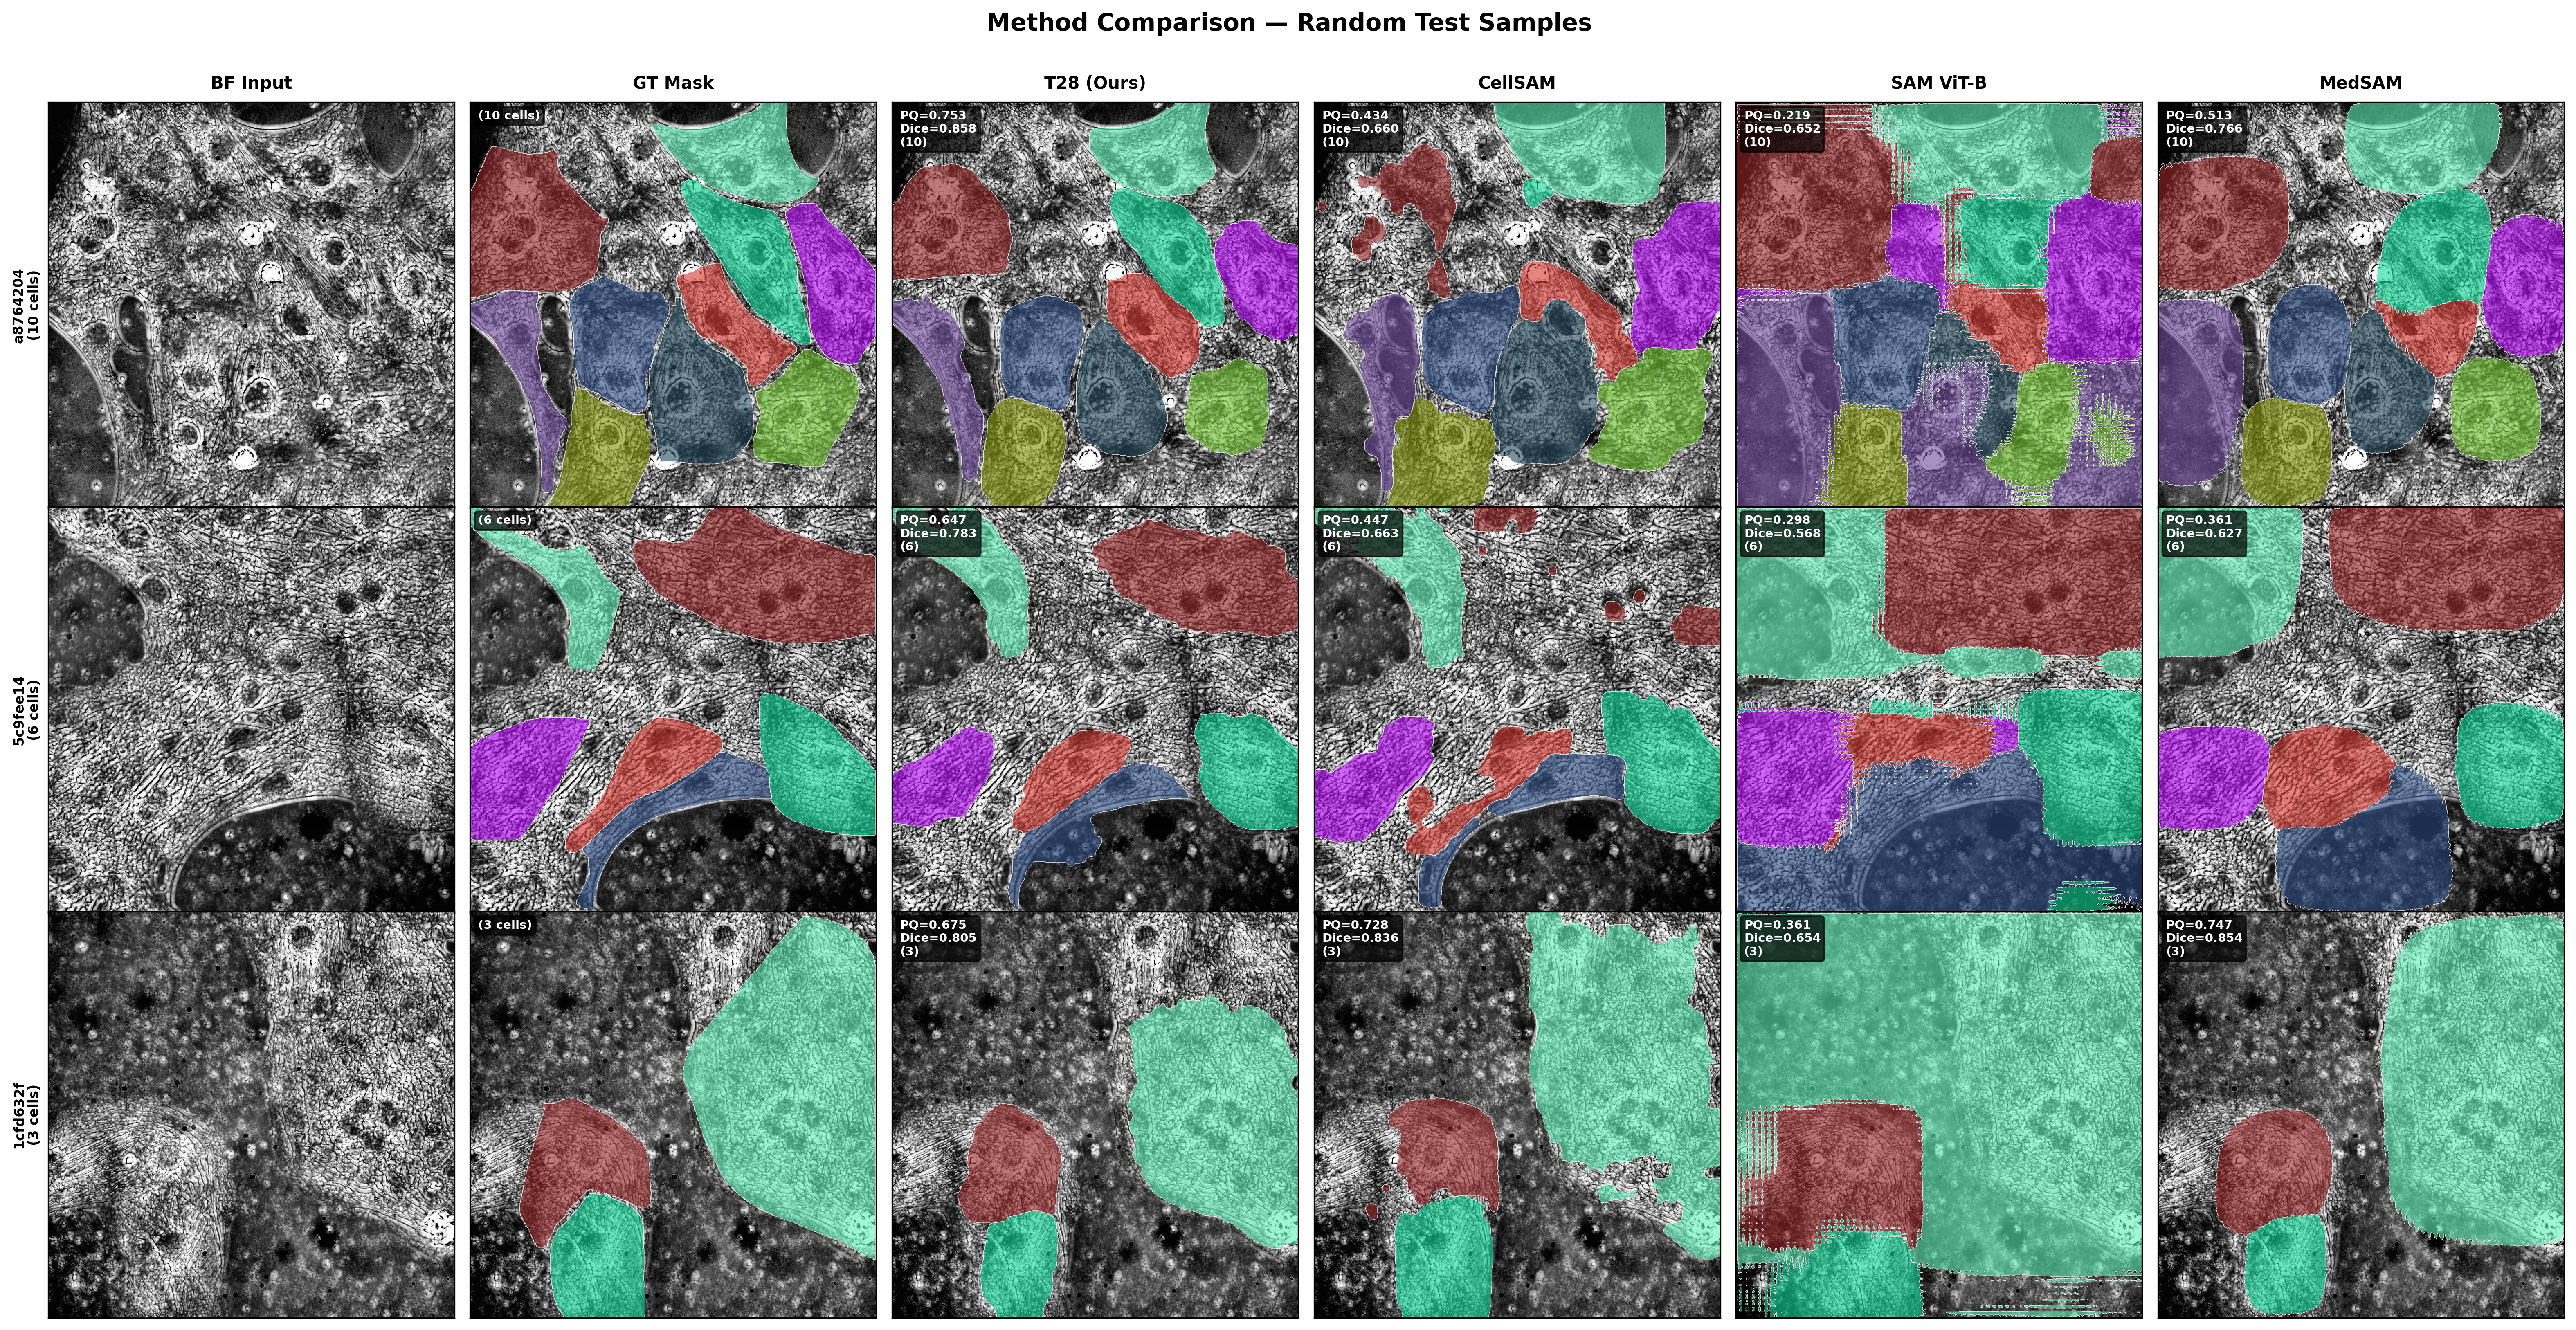
\includegraphics[width=\linewidth]{figures/paper_oracle_random3_no_cellpose_20260319.png}
  \caption{Oracle comparison on random test samples. With GT prompts, T28 yields high-quality masks, indicating that most end-to-end loss comes from detector prompt quality rather than mask refinement capacity.}
  \label{fig:t33g_t28_oracle_random3}
\end{figure}

\begin{figure}[t]
  \centering
  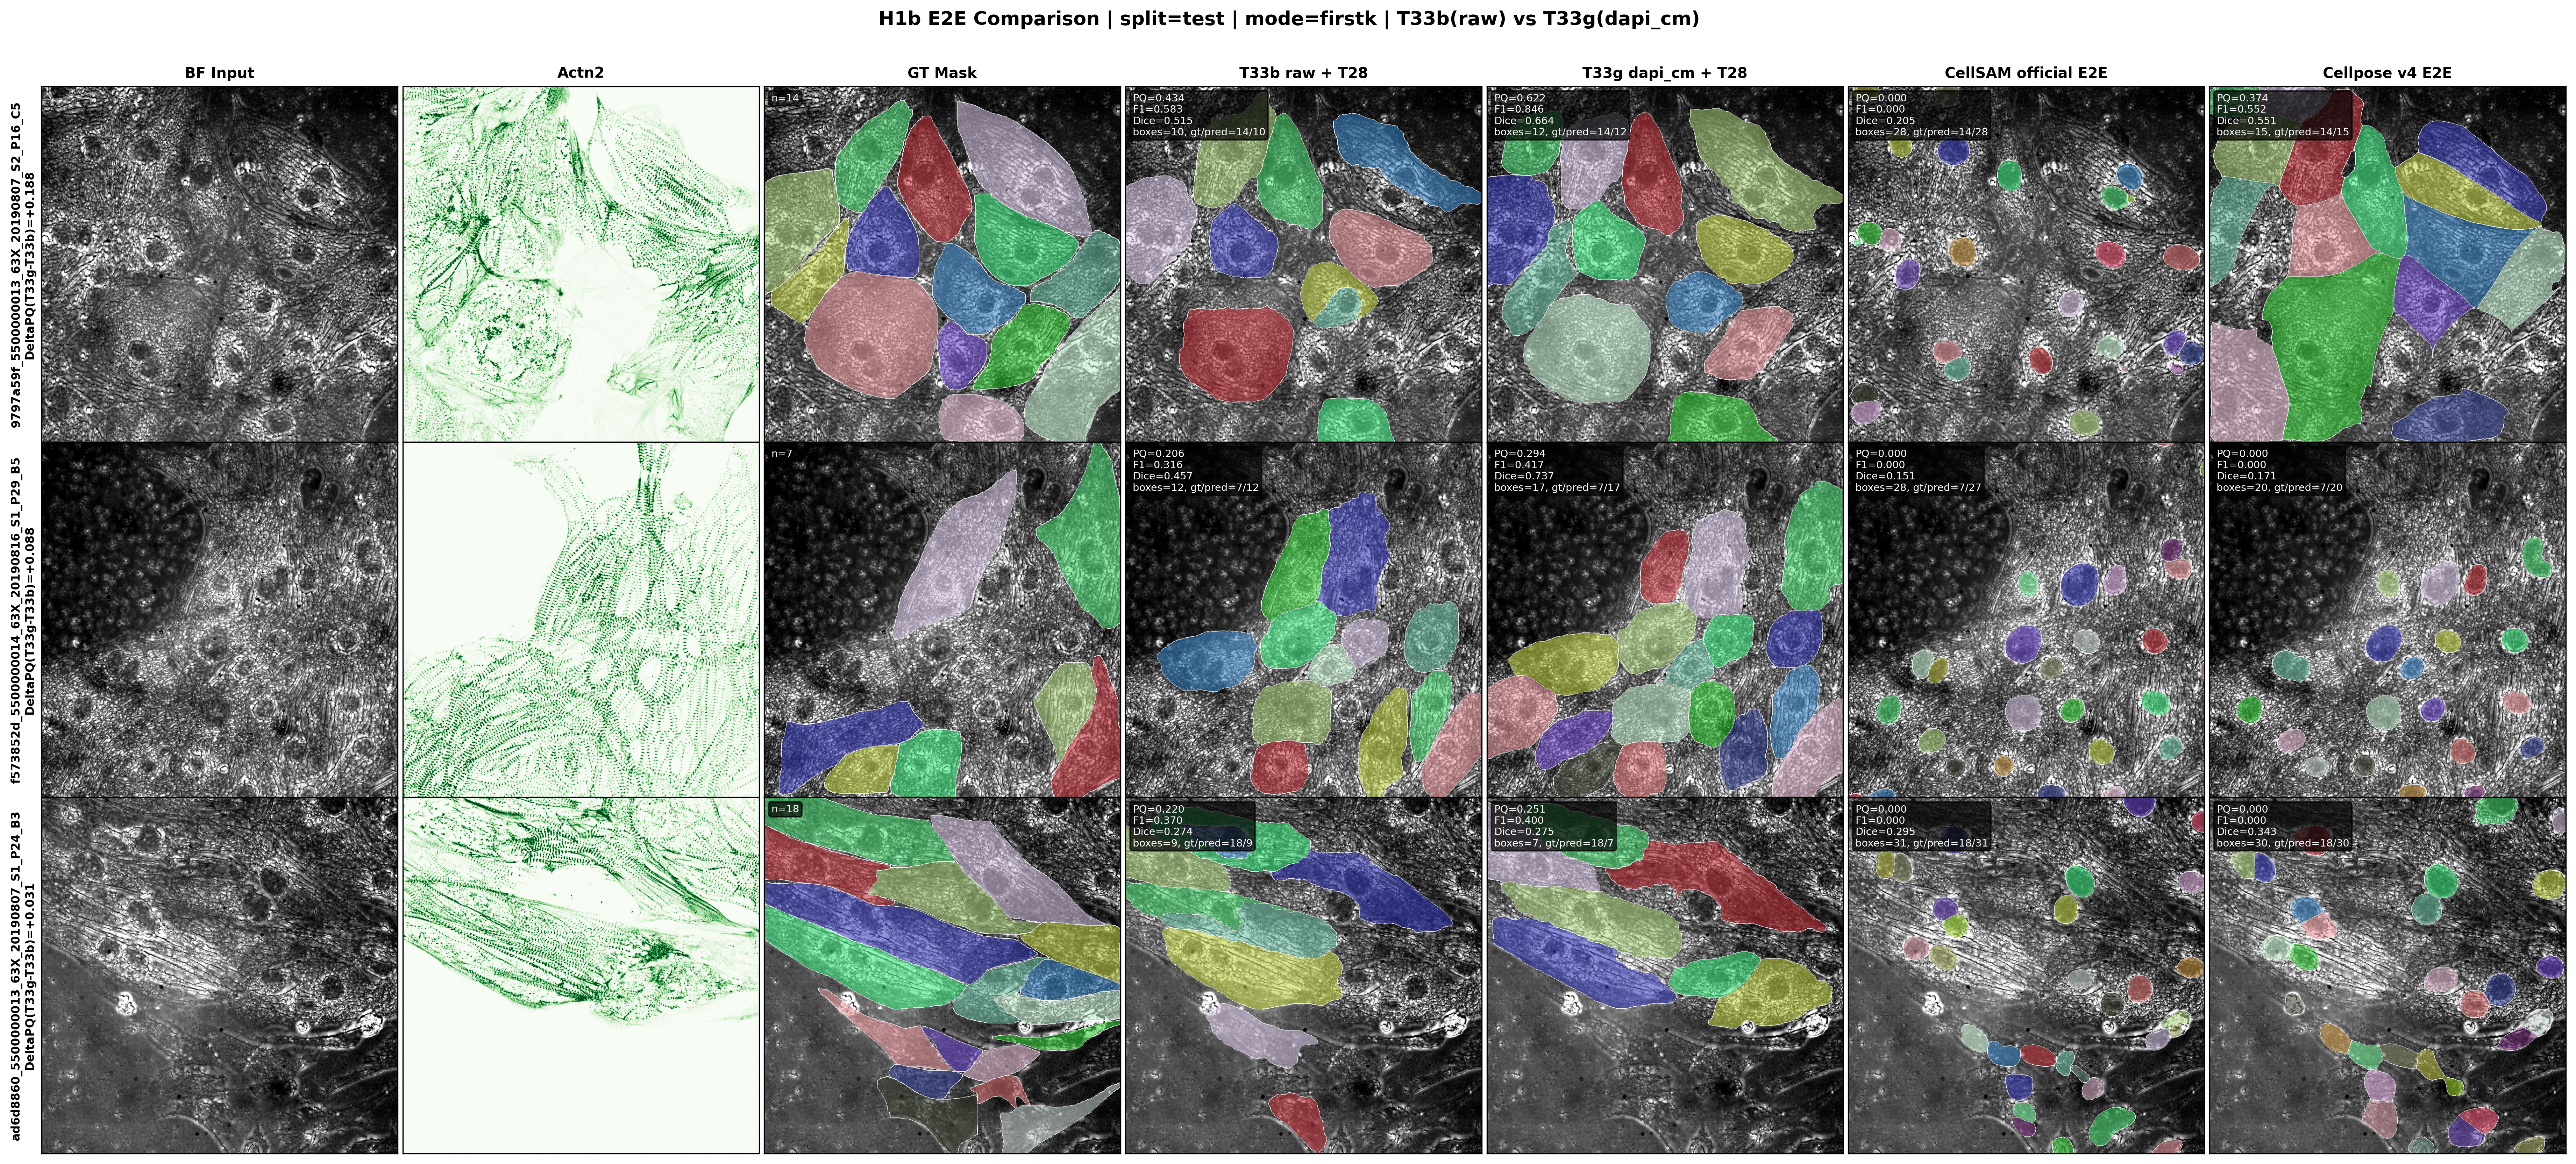
\includegraphics[width=\linewidth]{figures/t33g_t28_e2e_comparison_20260320.png}
  \caption{End-to-end qualitative comparison on three representative test samples. The T33g(dapi\_cm)+T28 route improves biologically plausible recovery over raw detector prompts while exposing known GT-v1 ambiguity cases.}
  \label{fig:t33g_t28_e2e_main}
\end{figure}

\begin{figure}[t]
  \centering
  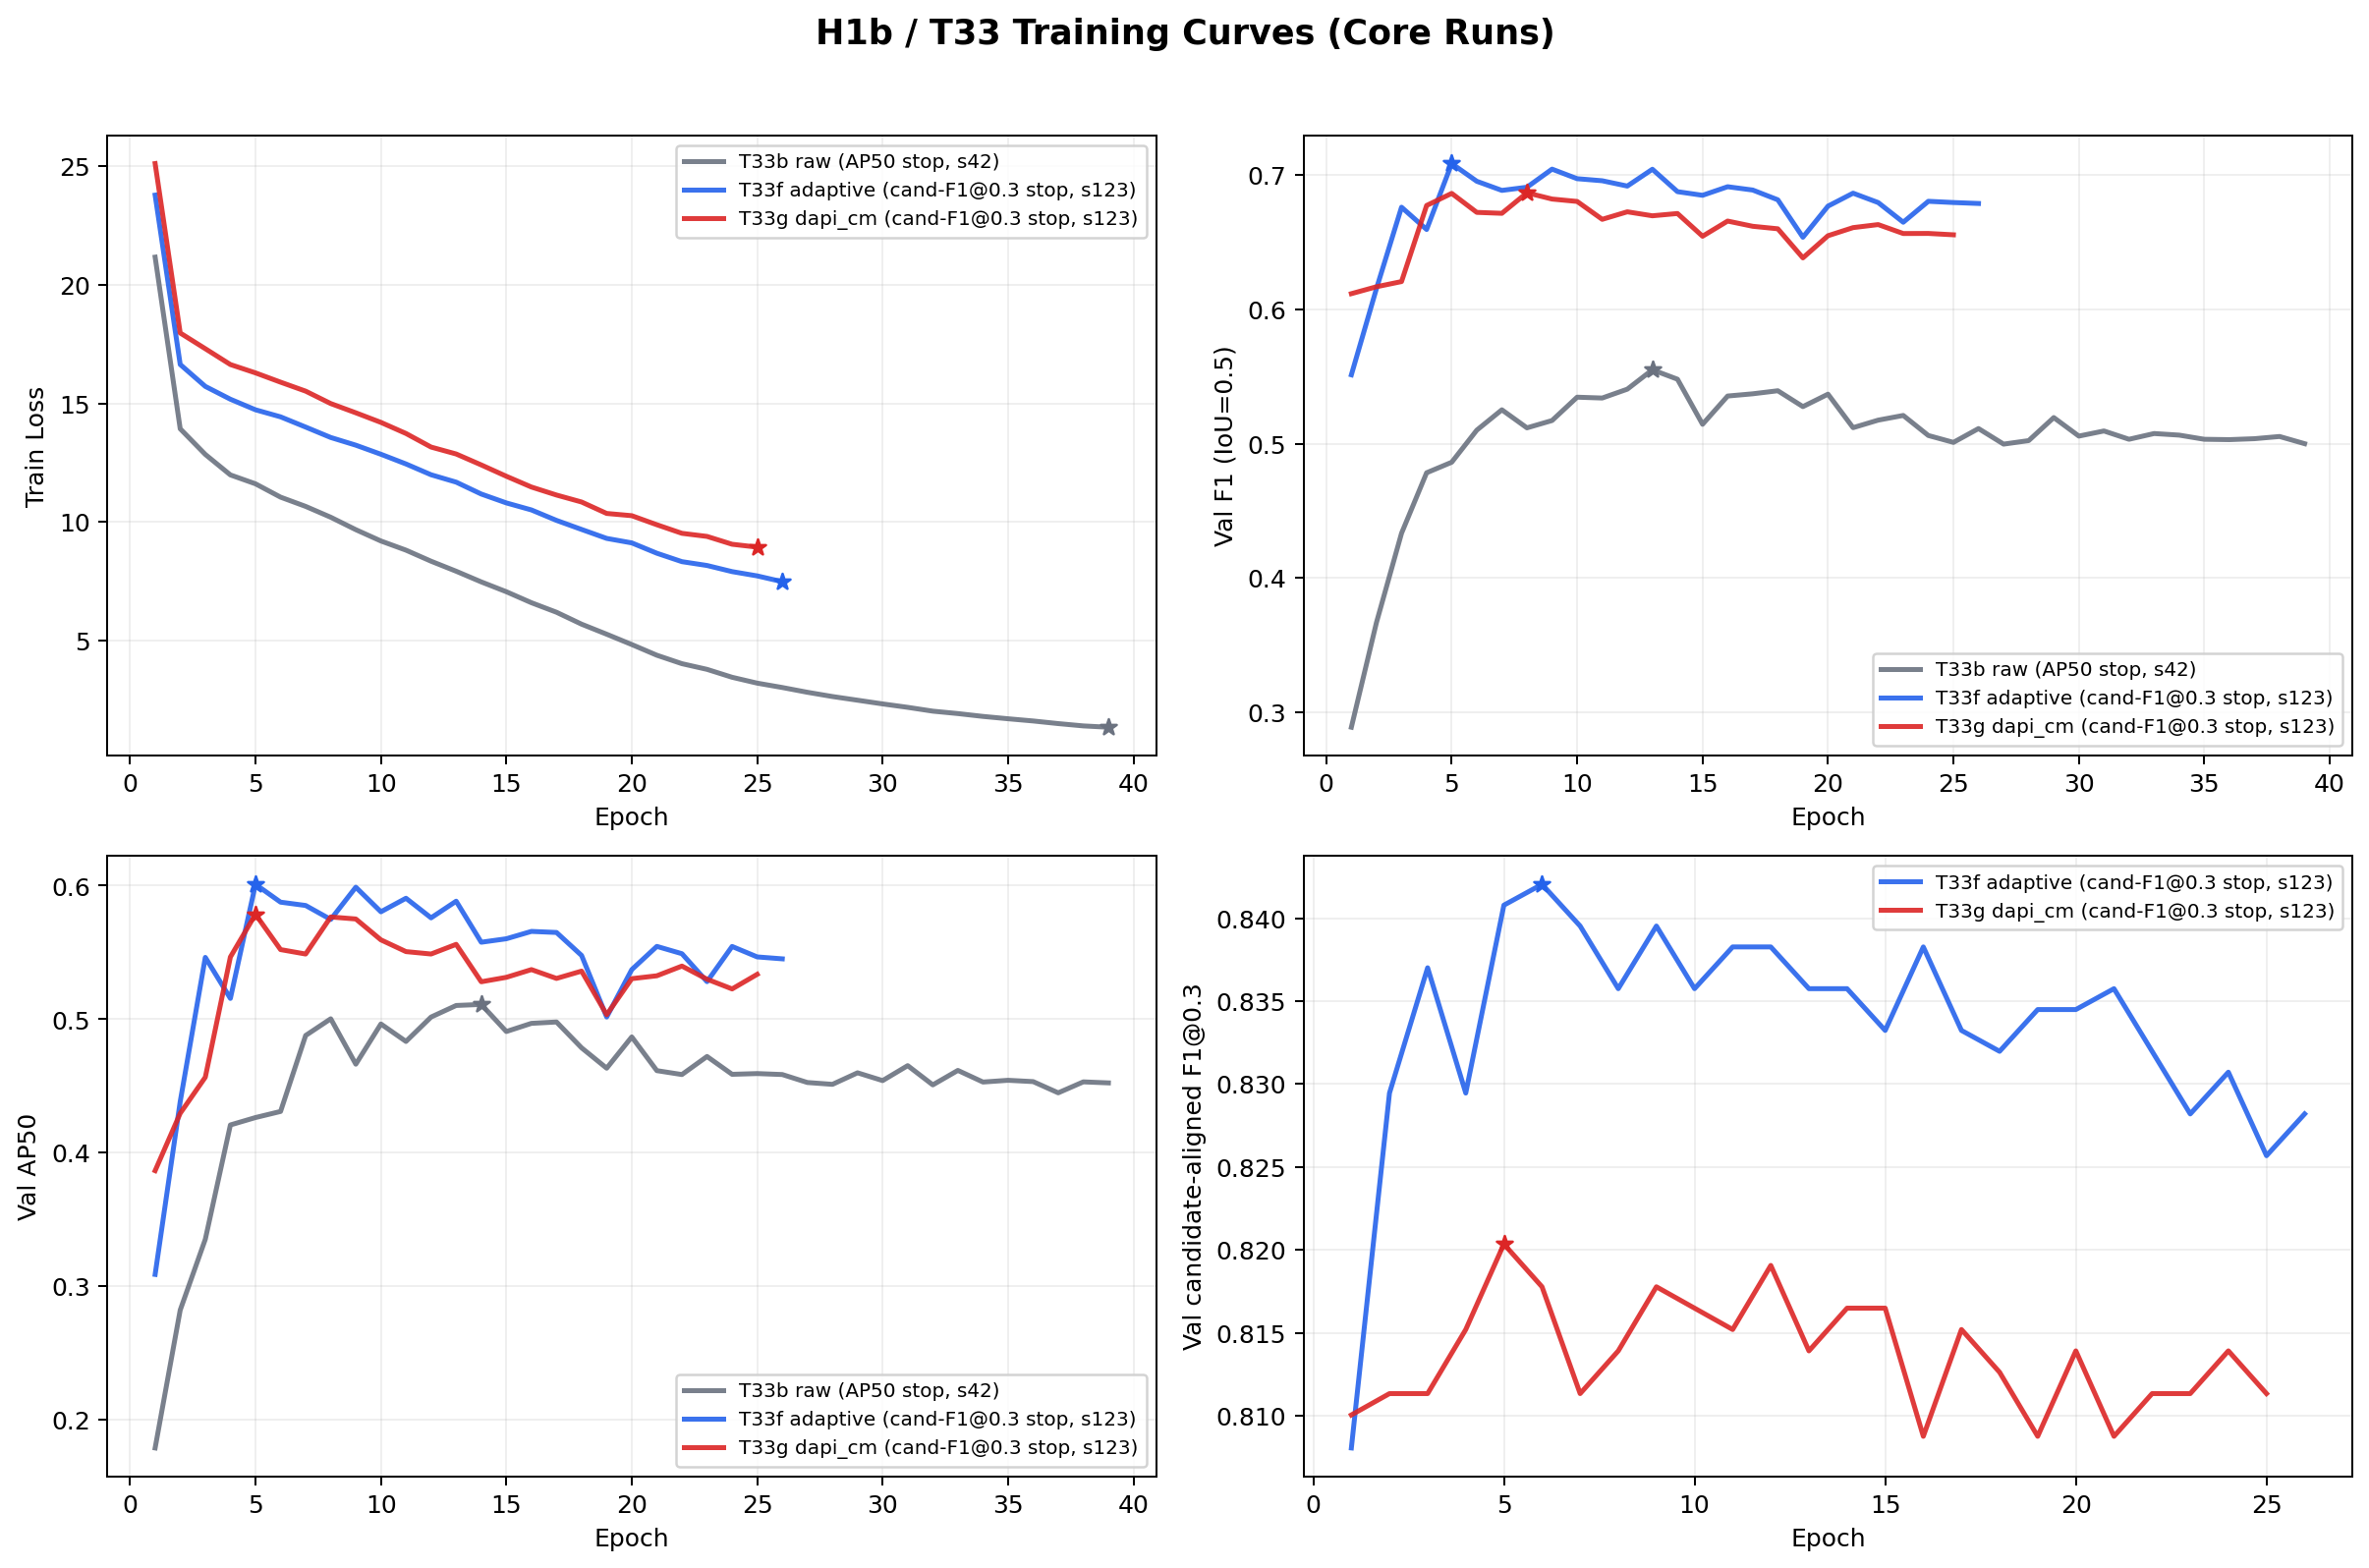
\includegraphics[width=\linewidth]{figures/t33_detector_training_curves_20260320.png}
  \caption{Training dynamics of T33 detector variants. Candidate-aligned F1@0.3 is the prior-aligned optimization target, while F1@0.5 and AP50 are auxiliary detector-quality monitors.}
  \label{fig:t33_detector_curves}
\end{figure}

GT-v1 contains likely missing or over-labeled instances in a small subset. This can suppress some end-to-end scores even when qualitative cardiomyocyte recovery is biologically plausible. Therefore, interpretation in Figure~\ref{fig:t33g_t28_e2e_main} is read jointly with metric evidence rather than as standalone proof.

\subsection{Prompt-Robustness Controls (Condensed Main-Text Anchor)}\label{prompt-robustness-controls-condensed-main-text-anchor}

To test whether simple mixed-prompt decoder retraining can close the Oracle-to-end-to-end gap, we ran three controls (\texttt{S2-E1/S2-E2/S2-E3}) initialized from the historical T27a route. The stable conclusion is negative: none of the controls improved end-to-end performance over the historical reference, and all reduced Oracle-side quality. Concretely, the best end-to-end control (\texttt{S2-E1}) still remains below the historical T27a reference by \texttt{0.024} PQ (\texttt{0.269} vs. \texttt{0.293}) and by \texttt{0.042} F1 (\texttt{0.455} vs. \texttt{0.497}), while also reducing Oracle PQ from \texttt{0.659} to \texttt{0.614}. This is an informative boundary result that supports the prompt-bottleneck diagnosis.

Therefore, the thesis does not promote mixed noisy-prompt decoder retraining as a main method branch. Detailed S2 settings and full metrics are reported in Appendix~B (\S\ref{s2-mixed-prompt-controls-supplementary-reference}).

\subsection{Provisional and Historical Observations}\label{provisional-and-historical-observations}

Not every useful experiment belongs in the main table. Some results are informative but should be written with weaker claims. Preliminary single-seed multi-channel observations are therefore kept in Appendix~B only, not promoted as body-level ablation evidence.

\subsubsection{T30 encoder adaptation is exploratory, not part of the current main result}\label{t30-encoder-adaptation-is-exploratory-not-part-of-the-current-main-result}

The T30 encoder-adaptation line (with historical T11 context) provided a modest positive signal. The best historical encoder-adaptation result reached \texttt{PQ\ =\ 0.494}, which is higher than Best Config but still below the current locked T27a \texttt{test73} reference. This keeps encoder adaptation as a future-work direction rather than a central thesis claim at the current stage.

\subsubsection{Neighbor/overlap exclusion losses are a negative result}\label{neighboroverlap-exclusion-losses-are-a-negative-result}

The P2-A experiments consistently degraded performance. The best delayed-activation setting still peaked before the extra losses became active, which indicates that naive repulsion-style losses conflict with the core segmentation objective on dense cardiomyocyte scenes.

This is worth keeping in the thesis because it shows that not all intuitively appealing structural losses are beneficial in practice.

\section{Discussion}\label{discussion}

\subsection{What Is Stable in the Current Evidence}\label{what-is-stable-in-the-current-evidence}

The current thesis already supports one stable central claim: cardiomyocyte-specific adaptation of the released CellSAM checkpoint is necessary, and the sealed T28 route provides a strong split-aware mainline. This conclusion is supported by the T28 dual-seed \texttt{val71} summary together with locked \texttt{test73} references against the released CellSAM checkpoint, the latest-version Cellpose rerun, and the MedSAM baseline. Therefore, the thesis can already argue for the value of task-specific adaptation without waiting for every side experiment to converge. For detector-driven integration, T28 is the fixed segmentation backend.

A second stable conclusion is that segmentation quality and prompting quality must be separated analytically. Under Oracle prompting, segmentation quality is strong. Under end-to-end prompting, performance drops sharply. This means the segmentation branch is no longer the main limiting factor once a correct box is available; the deployment bottleneck has shifted to detection quality.

This point is stronger than a single performance-number story because the baselines answer different questions rather than duplicating one another. Cellpose asks whether a strong generalist cell segmenter already transfers. SAM ViT-B asks whether generic promptable segmentation is enough without cell-domain adaptation. CellSAM-pretrained asks whether zero-shot cell-domain transfer is already sufficient. MedSAM asks whether large-scale medical pretraining dominates a cardiomyocyte-specific route. Taken together, the locked \texttt{test73} historical adaptation reference and the sealed \texttt{val71} T28 mainline support a multi-layer claim about task specificity, audited implementation, and evaluation discipline.

Under this framing, the value of the thesis is not that it simply trains another segmentation model. Its value is that it turns a released CellSAM pipeline into a domain-audited, prompt-aware, cardiomyocyte-specific system for a difficult adherent-cell setting with non-RGB biological channel semantics. The strongest methodological contributions are domain-aware input handling, prompt-quality-aware fine-tuning, and biology-prior-guided integration of DAPI and Actn2 cues with foundation segmentation.

\subsection{Released-Checkpoint Semantics Are Part of the Scientific Contribution}\label{released-checkpoint-semantics-are-part-of-the-scientific-contribution}

This thesis does not treat the released CellSAM checkpoint as a black box. Instead, it treats checkpoint semantics as part of the method. This is necessary because the public CellSAM release contains multiple internal branches, and the practical meaning of released-checkpoint segmentation inference is not recoverable from the paper narrative alone.

The published CellSAM paper describes a two-stage training scheme in which Stage 2 closes the gap between the adapted ViT features and the segmentation branch by freezing the ViT and the SAM mask decoder while fine-tuning the neck. However, the released checkpoint contains \texttt{model}, \texttt{model\_cp}, and \texttt{cellfinder} branches with globally different parameter sets. Therefore, the thesis draws a strict boundary between what is directly verifiable and what remains uncertain. We can verify which branch is used for inference and how the released checkpoint is structured. We cannot fully reconstruct the hidden training path that produced the public weights.

This distinction is not a minor implementation footnote. It affects reproducibility, baseline fairness, and the interpretation of every result that claims to represent the released CellSAM model. For this reason, the thesis explicitly anchors all released-checkpoint segmentation results to the \texttt{model\_cp} inference path and reports the remaining ambiguity as a limitation rather than hiding it.

\subsection{Detection Is the Main Deployment Bottleneck}\label{detection-is-the-main-deployment-bottleneck}

The Oracle-to-end-to-end gap is currently the clearest practical limitation of the system. Oracle performance shows that the segmentation branch can segment cardiomyocytes well when prompted with correct boxes. However, end-to-end performance remains much lower under automatic detection. This means the next large gain in practical usability is more likely to come from improving prompt quality than from making the segmentation decoder slightly stronger.

This observation also helps define the scope of the thesis. The thesis does not claim that the current pipeline is a fully solved end-to-end cardiomyocyte segmentation system. Rather, it claims that the segmentation branch has become strong enough that detection quality is now the dominant obstacle to deployment.

This is precisely why prompt-quality-aware adaptation and biology-prior-guided hybrid detection are methodologically grounded next steps rather than arbitrary engineering add-ons. The selected biology-prior detector branch (\texttt{T33g+T28}) should be read under this principle: it is chosen for biology-prior consistency (including Actn2-aware filtering), not because it is the detector-metric-optimal branch. This boundary is especially important under GT-v1 label ambiguity, where limited missing/over-labeled cases can distort strict metric ranking in end-to-end comparisons. At the same time, the sealed \texttt{S2-E3} result sharpens the boundary of that claim: switching the noisy source to frozen CellFinder prompts and early-stopping on validation E2E F1 still does not produce a positive turn. This suggests that the next practical gains are more likely to come from improving prompt generation itself than from another simple round of mixed noisy-box decoder fine-tuning.

\subsection{Limits of the Current Evidence Hierarchy}\label{limits-of-the-current-evidence-hierarchy}

Not all positive signals in the project carry the same evidential weight. T12 is useful because it has multi-seed support and explains why the loss evolution moved away from the original Phase 1 configuration. In contrast, the preliminary single-seed multi-channel observation retained in Appendix~B can only be treated as a weak directional signal, not as a locked body-level claim. Likewise, encoder-adaptation probes (for example T30, with historical T11 context) are interesting but remain exploratory rather than mainline.

Negative results also matter. The exclusion-loss experiments show that intuitively appealing structure-aware penalties can still harm performance on dense cardiomyocyte scenes. Keeping such results in the thesis improves credibility because it shows that the final method was not selected by selectively reporting only positive experiments.

\subsection{Future Work}\label{future-work}

There are five clear follow-up directions.

\begin{enumerate}
\def\labelenumi{\arabic{enumi}.}
\tightlist
\item
  Prioritize detector and prompt-generation quality over another simple round of mixed noisy-box decoder fine-tuning. The most direct route to closing the Oracle-to-E2E gap now appears to be better prompts, for example through biology-prior-guided hybrid detection or stronger detector-side query design, rather than assuming that mixed noisy boxes alone will unlock the gap.
\item
  Keep preliminary single-seed multi-channel evidence in appendix scope unless a multi-seed rerun confirms stability under the same reporting protocol.
\item
  Add training-dynamics assets for the final manuscript, centered on the sealed \texttt{T28} route (for example, stable training-curve reporting and split-consistent checkpoint selection evidence).
\item
  Treat mouse transfer, if mentioned, as a future adaptation problem rather than as a current result. A credible mouse pilot would require mouse labels, retuned detector priors, and a fresh evaluation of prompt quality rather than assuming direct zero-shot reuse from the current human hiPSC-CM pipeline.
\item
  Integrate a CellProfiler-assisted QC loop for annotation audit and detector-candidate validation (for example nucleus/cell association checks and morphology-based outlier flags), and evaluate whether this improves data quality control without conflating QC tooling with the primary end-to-end segmentation baseline \cite{carpenter2006cellprofiler,mcquin2018cellprofiler3}.
\end{enumerate}

\subsection{Concluding Remarks}\label{concluding-remarks}

Taken together, the current evidence supports a clear thesis claim: this work is not merely another fine-tuning result, but a domain-audited, prompt-aware, cardiomyocyte-specific adaptation framework for released cell foundation segmentation. Within that boundary, T28 establishes the sealed segmentation mainline, while the Oracle-to-E2E gap and the sealed \texttt{S2-E3} negative result show that the remaining bottleneck is no longer only the mask decoder, but the reliability of prompt generation in the full detection-to-segmentation pipeline. This, in turn, motivates prioritizing detector- and prompt-generation improvements, with noisy-box adaptation retained only as a constrained auxiliary hypothesis rather than the default next mainline.

\appendix
\section{Detailed Audit of the Released CellSAM Checkpoint}\label{detailed-audit-of-the-released-cellsam-checkpoint}

To clarify the actual structure of the released CellSAM checkpoint, we performed both code-level and parameter-level comparisons of its internal branches. The public checkpoint contains three relevant components: \texttt{model}, \texttt{model\_cp}, and \texttt{cellfinder}. For segmentation inference, the released implementation uses the \texttt{model\_cp} branch rather than \texttt{model}. In the same audited path, the mask decoder is called with \texttt{multimask\_output=False}, meaning that the practical segmentation route is the single-mask path rather than the multi-candidate SAM output mode.

Parameter-level comparison further shows that the checkpoint cannot be interpreted simply as a neck-only continuation from \texttt{model} to \texttt{model\_cp}. The branch \texttt{cellfinder.decode\_head.backbone.body} is exactly identical to \texttt{model.image\_encoder} after removing the neck (\texttt{171/171} matching parameter tensors), but entirely different from \texttt{model\_cp.image\_encoder} without the neck (\texttt{0/171}). Likewise, \texttt{model.image\_encoder} and \texttt{model\_cp.image\_encoder} are completely different once the neck is excluded (\texttt{0/171}). At the full-module level, \texttt{model} and \texttt{model\_cp} are globally distinct: the complete image encoder differs in \texttt{177/177} parameter tensors, the neck differs in \texttt{6/6}, the mask decoder differs in \texttt{120/120}, and the prompt encoder differs in \texttt{17/17}.

It is also important to distinguish architecture construction from weight loading. In the released code, \texttt{self.model\ =\ sam\_model\_registry{[}"vit\_b"{]}()} is instantiated first, and \texttt{self.model\_cp} is then created as a deep copy of this freshly constructed model. Therefore, before the released CellSAM checkpoint is loaded, \texttt{model} and \texttt{model\_cp} share the SAM ViT-B architecture and the same fresh initialization state, but they are not automatically the original Meta pretrained SAM checkpoint.

Relative to the original SAM ViT-B checkpoint, the released \texttt{model\_cp} branch preserves only a limited subset of parameters unchanged. The prompt encoder remains fully identical (\texttt{17/17} parameter tensors), while the mask decoder preserves \texttt{30/120} parameter tensors and changes the remaining \texttt{90/120}. The preserved mask-decoder tensors are concentrated in the IoU prediction head, the extra multimask hypernetwork branches, and a few attention \texttt{k\_proj.bias} terms. By contrast, the main single-mask output branch, the output upscaling path, the output tokens, and most transformer blocks are different. Because the released inference path uses \texttt{multimask\_output=False}, this pattern is consistent with further adaptation of the practical single-mask segmentation path, while some unused multi-output components may have remained unchanged.

This appendix supports two bounded claims that are safe for the thesis. First, the released checkpoint semantics must be audited rather than inferred from paper wording alone. Second, the released \texttt{model\_cp} segmentation branch is not the raw SAM mask decoder. What cannot be claimed from the public release alone is the exact hidden training procedure that produced these differences.

\section{Supplementary Preliminary Results}\label{supplementary-preliminary-results}

\subsection{S2 mixed-prompt controls (supplementary reference)}\label{s2-mixed-prompt-controls-supplementary-reference}

This subsection expands the condensed main-text statement in Chapter 5 for the mixed-prompt controls \texttt{S2-E1/S2-E2/S2-E3}. All three controls start from the historical T27a route and test whether simple noisy-prompt decoder retraining can improve end-to-end robustness.

{%
\begin{longtable}[]{@{}lcccccl@{}}
\toprule\noalign{}
Setting & Oracle PQ & Oracle RQ/F1 & Oracle BM-Dice & E2E PQ & E2E F1 & Note \\
\midrule\noalign{}
\endhead
\bottomrule\noalign{}
\endlastfoot
T27a reference & 0.659 & 0.960 & 0.800 & 0.293 & 0.497 & Historical baseline line \\
S2-E1 & 0.614 & 0.930 & 0.776 & 0.269 & 0.455 & Mixed prompts, clip ON \\
S2-E2 & 0.594 & 0.891 & 0.772 & 0.253 & 0.430 & Mixed prompts, clip OFF \\
S2-E3 & 0.599 & 0.903 & 0.770 & 0.174 & 0.288 & Mixed prompts, CellFinder noisy source, E2E-F1 early stop \\
\end{longtable}
}

Three points follow from these supplementary results. First, none of \texttt{S2-E1/S2-E2/S2-E3} improves over the historical T27a reference in end-to-end metrics. Second, all three controls reduce Oracle-side quality, indicating a robustness tradeoff rather than a net gain. Third, switching from Adaptive noisy prompts to a frozen CellFinder noisy source and early-stopping on validation E2E F1 (\texttt{S2-E3}) still fails to produce a positive turn. Therefore, these controls are retained as negative-but-informative boundary evidence, not as mainline method candidates.

\subsection{T18 preliminary single-seed multi-channel observations}\label{t18-preliminary-single-seed-multi-channel-observations}

T18 is retained for transparency because it provides a weak positive hint that fluorescence channels may help cardiomyocyte segmentation. However, the current evidence is based on a single seed and therefore does not meet the standard for a main-text ablation claim.

{%
\begin{longtable}[]{@{}
  >{\raggedright\arraybackslash}p{(\linewidth - 8\tabcolsep) * \real{0.3590}}
  >{\centering\arraybackslash}p{(\linewidth - 8\tabcolsep) * \real{0.1282}}
  >{\centering\arraybackslash}p{(\linewidth - 8\tabcolsep) * \real{0.2308}}
  >{\centering\arraybackslash}p{(\linewidth - 8\tabcolsep) * \real{0.1282}}
  >{\raggedright\arraybackslash}p{(\linewidth - 8\tabcolsep) * \real{0.1538}}@{}}
\toprule\noalign{}
\begin{minipage}[b]{\linewidth}\raggedright
Configuration
\end{minipage} & \begin{minipage}[b]{\linewidth}\centering
PQ
\end{minipage} & \begin{minipage}[b]{\linewidth}\centering
BM-Dice
\end{minipage} & \begin{minipage}[b]{\linewidth}\centering
AJI
\end{minipage} & \begin{minipage}[b]{\linewidth}\raggedright
Note
\end{minipage} \\
\midrule\noalign{}
\endhead
\bottomrule\noalign{}
\endlastfoot
Best Config (historical BF-only baseline) & 0.484 & 0.720 & 0.570 & 4-run mean \\
T18-A (BF + Actn2) & 0.496 & 0.724 & 0.573 & Single seed \\
T18-B (BF + Actn2 + DAPI) & 0.498 & 0.725 & 0.574 & Single seed \\
\end{longtable}
}

The direction is positive but small. Unless a second seed is added and the gain remains stable, T18 should be cited only as preliminary appendix evidence rather than as a locked thesis conclusion.

\subsection{T28 Mechanistic Supplementary Visualizations}\label{t28-mechanistic-supplementary-visualizations}

The following visualizations are retained as mechanism-oriented supplementary evidence. They are useful for interpreting model behavior but are not used as primary quantitative proof.

\begin{figure}[t]
  \centering
  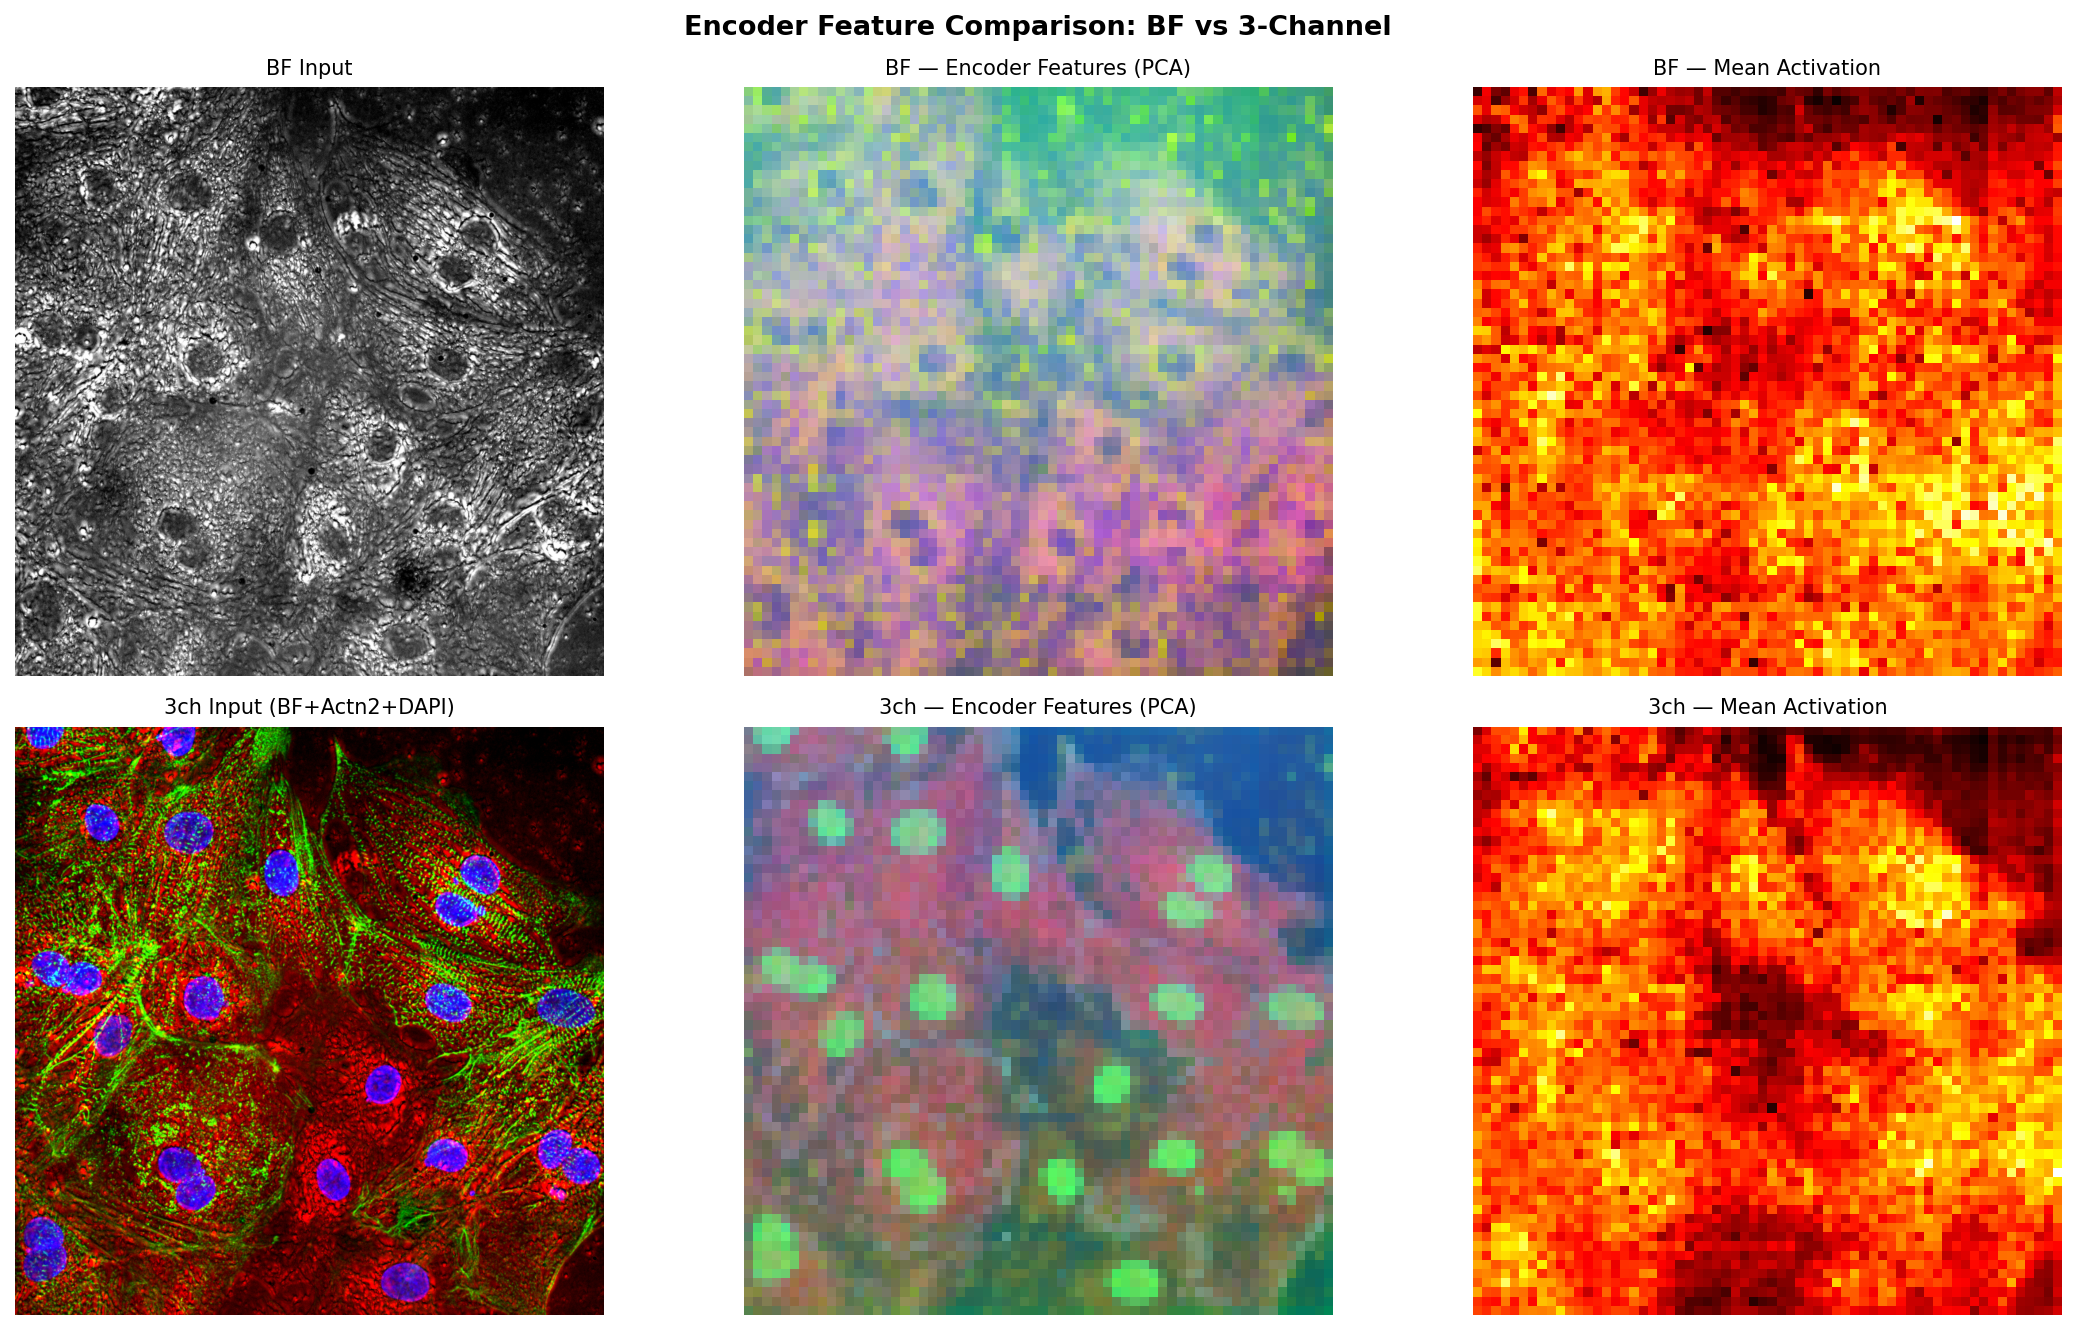
\includegraphics[width=\linewidth]{figures/t28_attention_heatmap_9797a59f_5500000013_63X_20190807_S2_P16_C5.png}
  \caption{T28 encoder activation heatmap under BF-replicate versus three-channel input. This figure provides qualitative representation-level evidence only.}
  \label{fig:app_t28_encoder_heatmap}
\end{figure}

\begin{figure}[t]
  \centering
  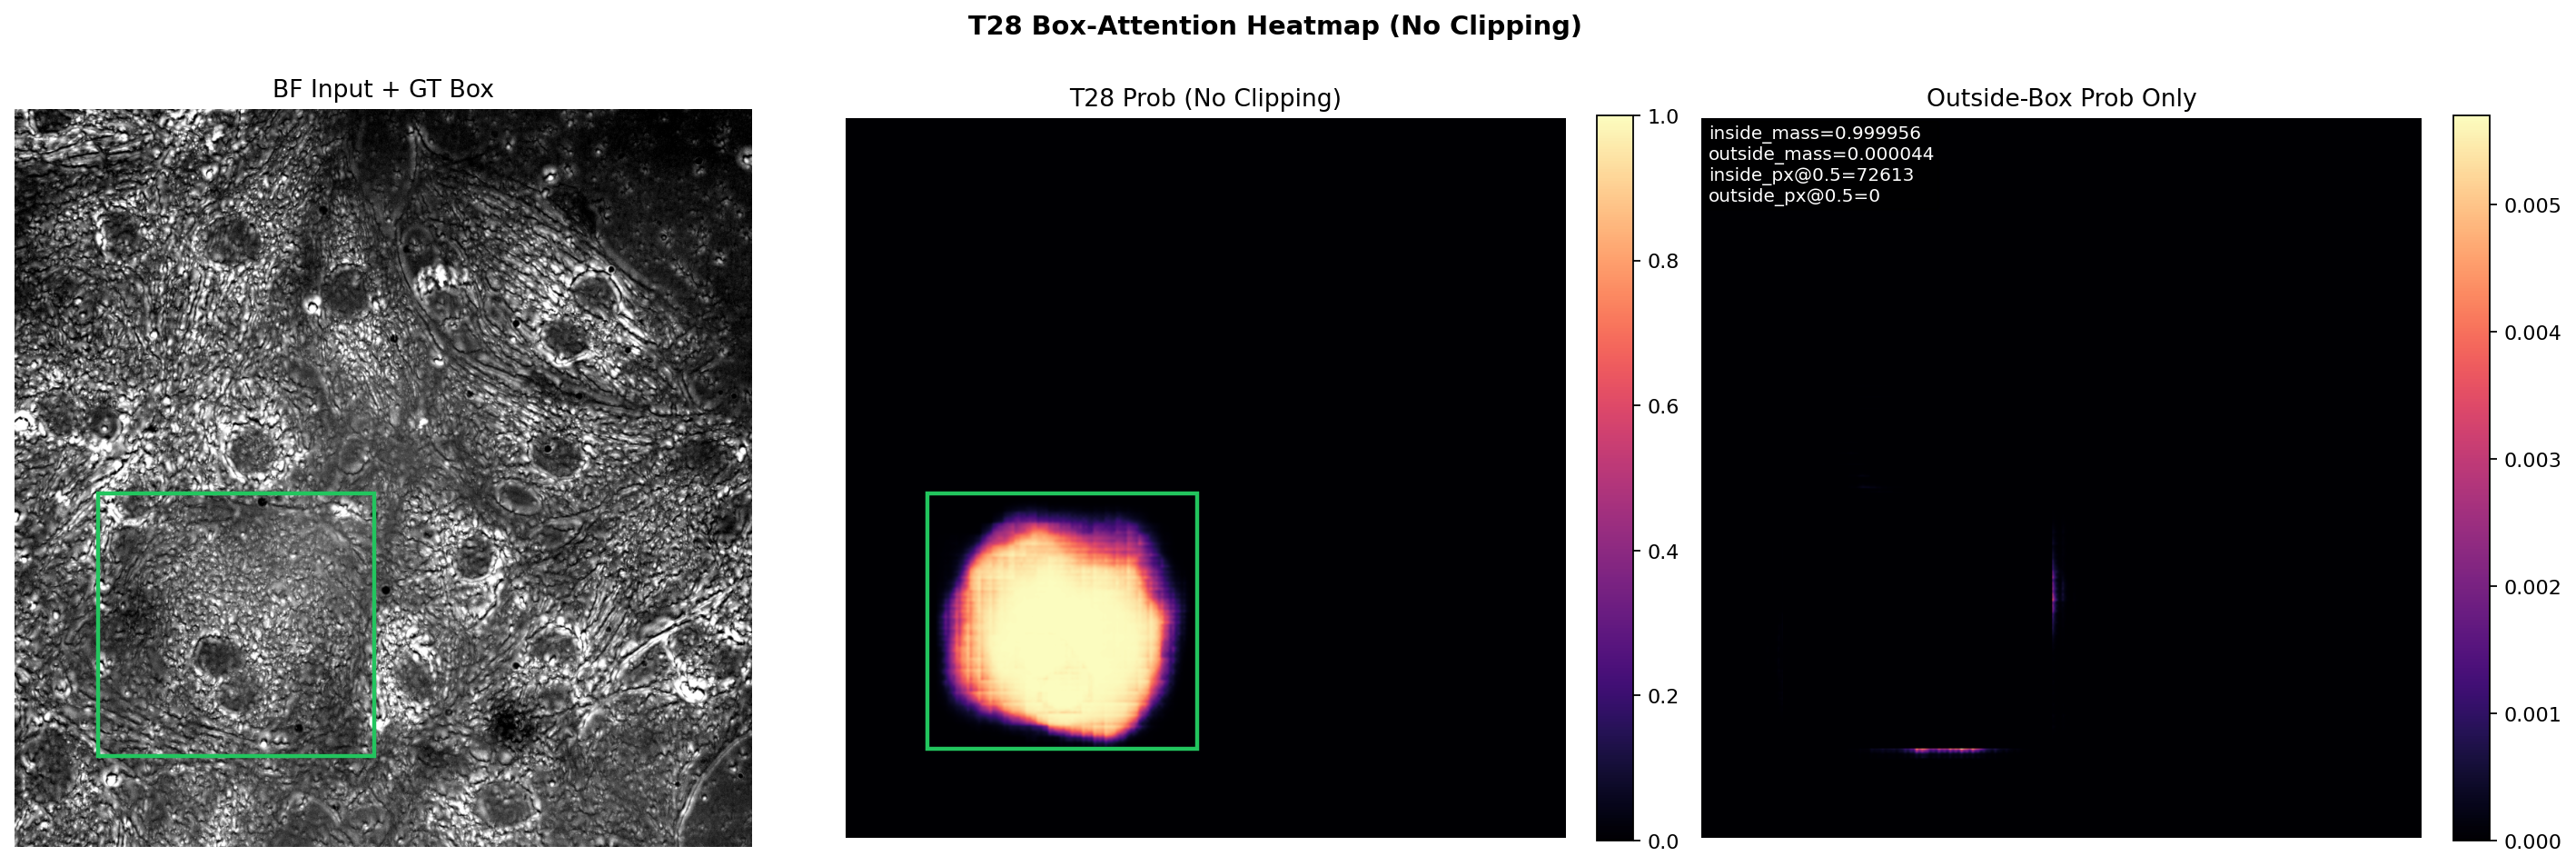
\includegraphics[width=\linewidth]{figures/t28_box_attention_9797a59f_5500000013_63X_20190807_S2_P16_C5_cell10.png}
  \caption{T28 box-outside probability heatmap (no clipping) on one representative sample. The outside-box probability mass is low in this case, which is consistent with weak clipping sensitivity under GT-box settings.}
  \label{fig:app_t28_box_heatmap}
\end{figure}

Both figures are interpreted as sample-level explanatory diagnostics. They should be read together with main-text metrics rather than as independent claims about full-dataset behavior.

% !TEX root = ../main.tex
\section{Scope and Transfer Notes}\label{scope-and-transfer-notes}

\subsection{Human--Mouse Transfer Boundary and Species-Specific Differences}\label{appendix-human-mouse-transfer-boundary}

This appendix records the scope boundary behind the main thesis claims. All locked experiments and all headline conclusions in the main text are restricted to \textbf{human hiPSC-derived cardiomyocytes}. Mouse transfer is scientifically relevant, but it remains an adaptation question rather than a supported zero-shot generalization claim in the current evidence tier.

Table~\ref{tab:human_mouse_gap} summarizes the species- and preparation-level differences that are most likely to affect the present detector-to-segmenter pipeline.

\begin{table}[htbp]
\centering
\small
\caption{Human hiPSC-CM versus typical mouse cardiomyocyte settings: expected impact on this thesis pipeline.}
\label{tab:human_mouse_gap}
\begin{tabular}{p{0.16\linewidth}p{0.25\linewidth}p{0.25\linewidth}p{0.26\linewidth}}
\toprule
Dimension & Current thesis setting (human hiPSC-CM) & Typical mouse setting & Expected impact on pipeline \\
\midrule
Maturation & Immature/fetal-like state is common & Adult primary preparations are often more mature & Distribution shift in texture, boundary statistics, and morphology priors \\
Shape & Spread, anisotropic, irregular monolayer morphology & Adult isolated CMs are often rod-shaped \cite{li2014isolation_mouse_cm} & Detector box priors and postprocessing thresholds require retuning \\
Nucleation & Mono-nuclear or mixed immature states are common & Bi-/multi-nucleated cardiomyocytes are more frequent in mature preparations \cite{ahmed2020hipscm_maturation} & Nucleus-to-cell association logic becomes less reliable if reused unchanged \\
Electrophysiology context & Human hiPSC-CM physiology and maturation trajectory & Rodent cardiac electrophysiology differs from human \cite{joukar2021rodent_human_ecg} & Species mismatch limits direct transfer claims from human-trained priors \\
Marker behavior & Actn2 and DAPI reflect human hiPSC-CM culture context & Marker appearance varies with species and preparation & Prompt quality and candidate filtering rules need species-specific recalibration \\
\bottomrule
\end{tabular}
\end{table}

A credible mouse-transfer route should therefore include at least: (i) mouse-domain zero-shot audit, (ii) detector-prior retuning, and (iii) mouse-specific decoder fine-tuning under the same split-aware evaluation protocol.


\clearpage
\bibliographystyle{unsrt}
\bibliography{references}
\addcontentsline{toc}{section}{References}

\end{document}
